\documentclass[letterpaper, 12pt]{article}
\usepackage[french, english]{babel}

\usepackage{amsmath,amsfonts,amsthm,amssymb,graphicx,wasysym,multirow}
\usepackage[latin1]{inputenc}

\usepackage{hyperref}

\pagestyle{plain}

\setlength{\topmargin}{-2cm}
\setlength{\textheight}{23.5cm}
\setlength{\textwidth}{18cm}
\setlength{\oddsidemargin}{-1cm}
\setlength{\parindent}{0pt}

\begin{document}

3000-- The Egyptians only knew how to add and multiply by 2. They used the following symbols to calculate.\\

\begin{center}
\begin{tabular}{|c|c|c|}
\multicolumn{3}{c}{\bf Egyptian Symbols}\\[2mm] \hline
{\bf Symbol} & {\bf Meaning} & {\bf Quantity}  \\ \hline \hline
 & & \\

\includegraphics[scale=0.8]{Hiero1.eps} & stick & 1\\[4mm] \hline
 & & \\

\includegraphics[scale=1.6]{Hiero10.eps} & basket handle & 10\\[4mm] \hline
 & & \\

\includegraphics[scale=1.5]{Hiero100.eps} & Papyrus roll & 100\\[4mm] \hline
 & & \\
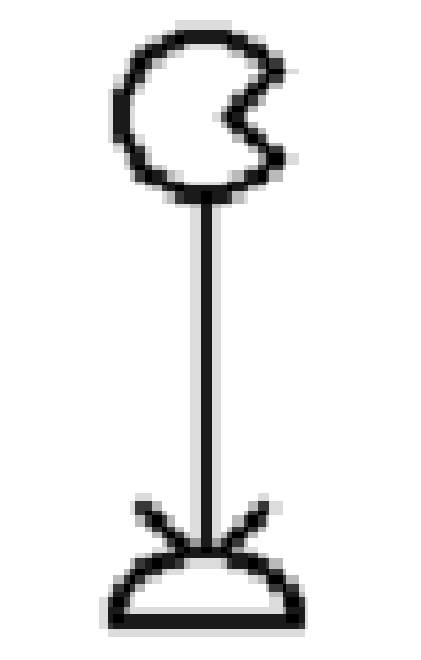
\includegraphics[scale=0.08]{Hiero1000.eps} & Lotus flower & 1000\\[4mm] \hline
\multicolumn{3}{c}{}\\
\end{tabular}
\end{center}

\ Calculate the following sum by referring to the table:
\begin{center}
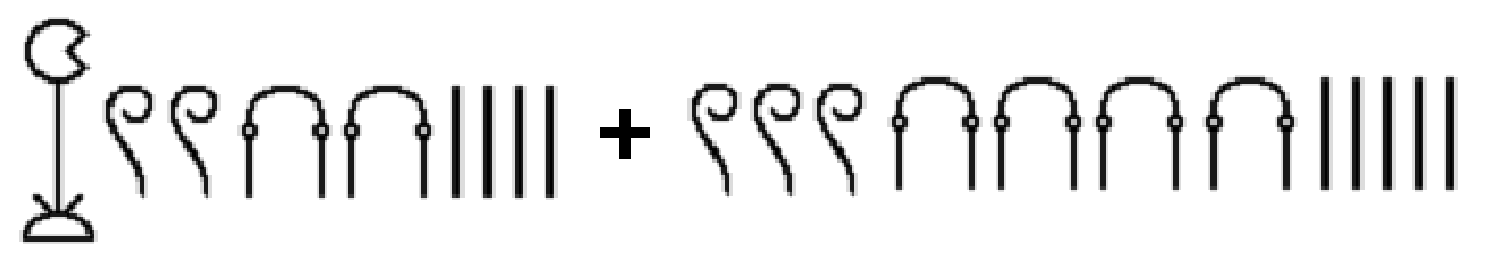
\includegraphics[scale=0.35]{1569.eps}\\
\end{center}

Answer: $1569$\\

Explanation :\\
The Lotus flower is worth $1000$, the Papyrus roll $100$, the basket handle $10$ and the stick $1$.\\
Therefore, the first group of symbols:\\
\begin{center}
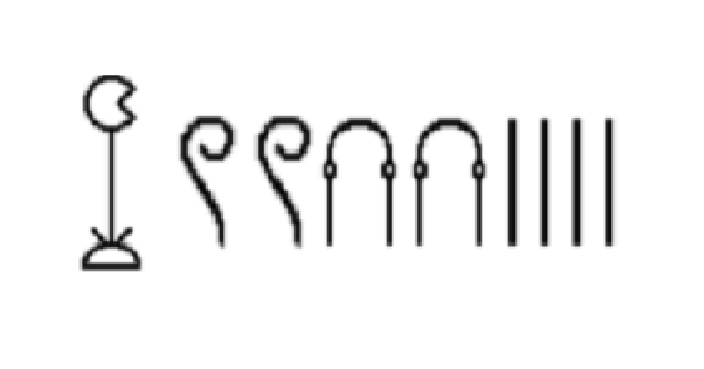
\includegraphics[scale=0.35]{1224.eps}\\
$= 1000 + 2 \times 100 + 2 \times 10 + 4 \times 1 = 1224$.\\[4mm]
\end{center}
And the second:\\
\begin{center}
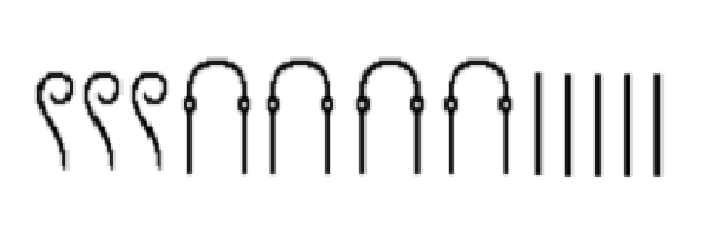
\includegraphics[scale=0.35]{345.eps}\\
$= 3 \times 100 + 4 \times 10 + 5 \times 1  = 345$.\\[4mm]
\end{center}
Thus, the answer is: $1224 + 345 = 1569$.\\

Images taken from the website: \href{http://fr.wikipedia.org/wiki/Num\%C3\%A9ration \%C3\%A9gyptienne}{fr.wikipedia.org/wiki/Num\'eration \'egyptienne}\\



3001-- Among the following symbols, which one represents a number written in Babylonian?\\


a) :\textsf{P}\\
b) XXIV\\
c) 
\includegraphics[scale=0.1]{30.eps} \includegraphics[scale=0.1]{5.eps}\\
d) 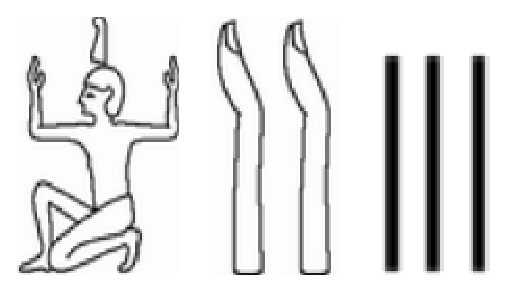
\includegraphics[scale=0.15]{nombregyptien.eps}\\

Answer: c)\\

Explanation:\\
:\textsf{P} is a grimace in chatroom language.\\
XXIV is the number $24$ in Roman numerals.\\

\includegraphics[scale=0.1]{30.eps} \includegraphics[scale=0.1]{5.eps} is the number 35 in written Babylonian.\\
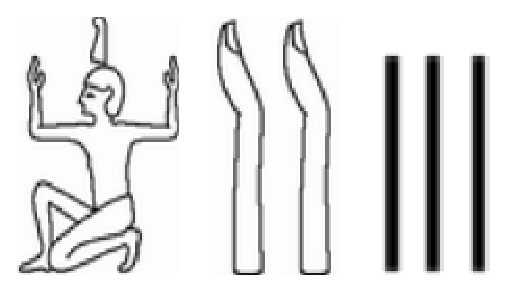
\includegraphics[scale=0.12]{nombregyptien.eps} is the number 1 020 003 in Egyptian writing.\\
The correct answer is therefore c).\\

Images taken from the website : \href{http://fr.wikipedia.org}{fr.wikipedia.org}\\

\og$\perp$\fg \

%{\bf \textsf{animation : bonhomme d\'eguis\'e en romain appara\^it, poings sur les hanches, chevelure au vent}}\\
3002-- How much is the following Roman numeral worth: MMCDLXIV ?\\

a) $2464$\\
b) $2666$\\
c) $5444$\\
d) $5466$\\

Answer: a)\\

Explanation:\\
\begin{center}
\begin{tabular}{|c|c|}
\multicolumn{2}{c}{\bf List of numerals}\\[2mm] \hline
{\bf Roman numerals} & {\bf Amounts} \\[1mm] \hline \hline
M & 1000 \\[1mm] \hline
D & 500 \\[1mm] \hline
C & 100 \\[1mm] \hline
L & 50 \\[1mm] \hline
X & 10 \\[1mm] \hline
V & 5 \\[1mm] \hline
I & 1 \\[1mm] \hline
\multicolumn{2}{c}{}\\
\end{tabular}\og$\perp$\fg \
\end{center}
In order to form a number, a letter is written in descending order according to its value. For example, MI is written $1001$.  Each letter's value is added to form the number, unless
\begin{center}
I is to the left of V or X,\\
X is to the left of L or C,\\
C is to the left of D or M.\\
\end{center}
In this case, the{\small(598-668)} letter to the left is subtracted (for example: XL = L -- X = $50 - 10 = 40$).\\

Therefore, MMCDLXIV = $1000 + 1000 + (500 - 100) + 50 + 10 + (5 - 1) = 2464$. The correct answer is a).\\



%{\bf\textsf{animation : le petit bonhomme compte ses doigts}}\\
3003-- The numbers `` $0, 1, 2, 3, 4, 5, 6, 7, 8, 9$ '' \ are of Arabic origin. Why did the Arabs decide to use the decimal system (based on 10) in mathematics?\\

a) Each Arab owned 10 sheep.\\
b) 10 was a sacred religious number\\
c) Humans have 10 fingers each.\\
d) In the old days, the Royal Family always had 10 children.\\

Answer: c)\\

Explanation:\\
All research leads experts to believe that the decimal system comes from the possibility to count with our 10 fingers. The English synonym for finger, "digit", comes from the latin word "digitus", which means "finger". The correct answer is therefore c).\\



3004-- When was the first time that arithmetic symbols were used in mathematics? (for example: $+, -, \times , \leq , \geq $)\\

a) during the prehistoric era\\
b) $1000$ BC, during the Babylonian era\\
c) during the XIV century, at the beginning of the Renaissance era\\
d) during the XX century\\

Answer : c)\\

Explanation :\\
Before and throughout the Ancient Greek era, there weren't any symbols to represent arithmetic operations and relationships. People wrote out all their problems and solutions into words. It wasn't until the beginning of the Renaissance period that one could see the first symbols written out by hand. Thus, the correct answer is c).\\



3005-- How many different symbols exist to represent multiplication?\\

a) 1\\
b) 2\\
c) 3\\
d) 4\\

Answer: d)\\

Explanation :\\
\begin{center}
\begin{tabular}{|l|c|c|}
\multicolumn{3}{c}{\bf Evolution of the multiplication symbol}\\[2mm] \hline
{\bf Date of appearance} & {\bf Symbol} & {\bf Example} \\[1mm] \hline \hline
{IX century} & {juxtaposition} & $3 \, (4 + 5)$ \\[1mm] \hline
beginning XVII century & $\times$ & $3 \times (4 + 5)$ \\[1mm] \hline
1698 & $\cdot$ & $3 \cdot (4 + 5)$ \\[1mm] \hline
today (more common in information technology lingo) & $\ast$ & $3 \ast (4 + 5)$ \\[1mm] \hline
\multicolumn{3}{c}{}
\end{tabular}B
\end{center}
The symbol $\cdot$ was created because mathematicians of that time period were worried about confusion between $\times$ and the variable $x$. It is for that reason that there are 4 existing symbols that represent multiplication. The correct answer is d).\\



3006-- How many different division symbols are there in mathematics??\\

a) 1\\
b) 2\\
c) 3\\
d) 4\\

Answer: d)\\

Explanation :\\
\begin{center}
\begin{tabular}{|c|c|l|}
\multicolumn{3}{c}{\bf Evolution of the division symbol}\\[2mm] \hline
{\bf Symbol} & {\bf Example} & {\bf Notes} \\ \hline \hline
$\div$ & $3 \div 5$ & appeared for the first time in a Swiss book in the 17th century \\[1mm] \hline
$/$ & $3 / 5$ & first way to write a fraction\\[1mm] \hline
$-$ & $\frac{3}{5}$ & another way to write a fraction \\[1mm] \hline
$:$ & $3:5$ & ratio \\[1mm] \hline
\multicolumn{3}{c}{}
\end{tabular}
\end{center}
Thus, there are four ways to write the division symbol. The correct answer is d).\\



3007-- What important mathematic discovery do we use now on a daily basis that in the olden days was difficult to understand?\\

a) Counting on our fingers\\
b) Addition\\
c) Geometry\\
d) the number zero\\

Answer: d)\\

Explanation:\\
Even if all of these discoveries were important, one of them was by far the most difficult to understand.\\
In the IX century, Indians defined an important mathematical concept: the `` \emph{zero} ''. Like most of the time, numbers were only used to count objects, it was difficult to associate the concept "there is no object" (there is nothing to count) to a number.  They must have seen the numbers $1, 2, 3, ...$ as objects and not only as numeric adjectives. Soon thereafter, these numbers had to exist even if there was nothing to count. And only then did  the number zero come into existence. The correct answer is d). It was the mathematician Al-Khwarizmi who spread his idea of the number zero to Western Europe.\\
\begin{center}
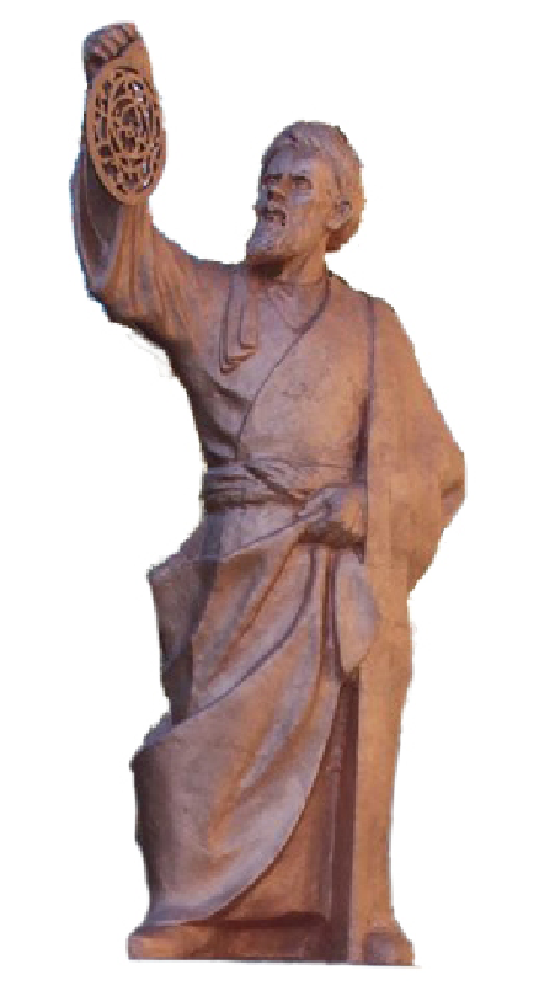
\includegraphics[scale=0.25]{Al-Khwarizmi.eps}\\
\emph{{\small Al-Khwarizmi}}\\
\href{http://fr.wikipedia.org/wiki/Al-Khwarizmi}{fr.wikipedia.org/wiki/Al-Khwarizmi}\\[5mm]
\end{center}



3008-- In the XVII Century, a solution was proposed to resolve a second degree equation in the following manner: `` \emph{Move all the terms to the same congruent side in such a way that they equal zero.} ''
\begin{eqnarray*}
x^{2} + 2 &=& 3x\\
x^{2} - 3x +2 &=& 0
\end{eqnarray*}\\
`` \emph{Factor equation and place each factor equal to zero.} ''
\begin{eqnarray*}
x^{2} - x - 2x +2 = 0\\
x\cdot(x - 1) - 2\cdot(x - 1) = 0\\
(x - 1)\cdot(x - 2) = 0\\
(x - 1) = 0 \ \ \textrm{et} \ \ (x - 2) = 0\\
x = 1 \ \ \textrm{et} \ \ x = 2
\end{eqnarray*}\\
Which English mathematician came up with this idea?\\

a) Andrei Markov\\
b) John Pell\\
c) Thomas Harriot\\
d) Zenodore\\

Answer: c)\\

Explanation:\\
Andrei Markov is the name of a Russian mathematician and a Russian hockey player. John Pell is an English mathematician who is known for the Pell's Equation. It was Thomas Harriot who came up with the idea of how to solve second degree equations. This principle is sometimes called "The Harriot Principle". Thus, the correct answer is c).\\
\begin{center}
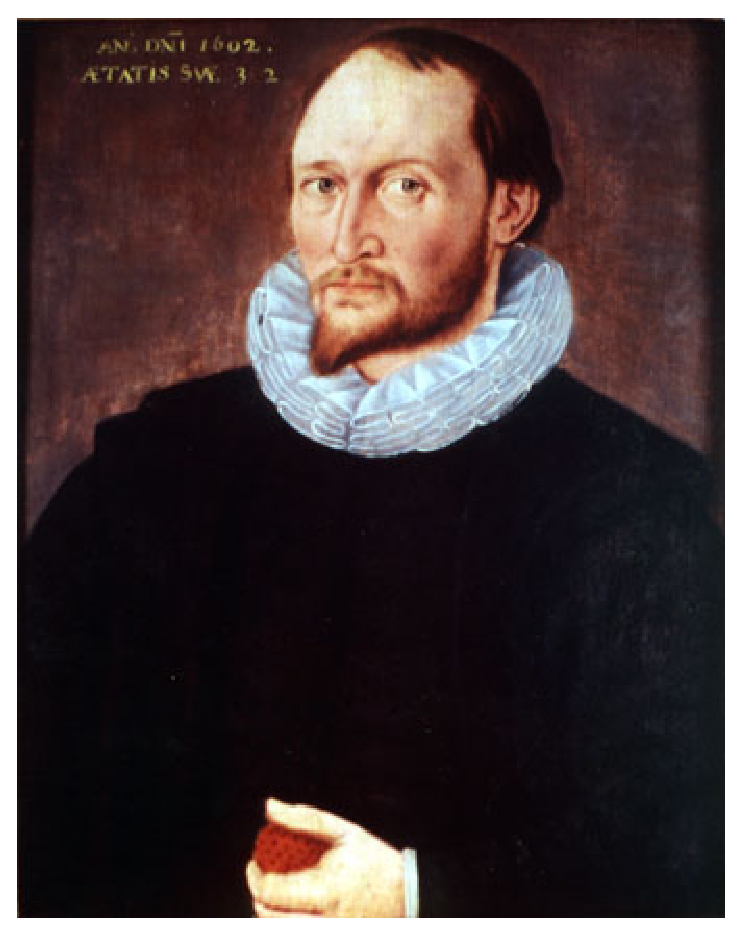
\includegraphics[scale=0.25]{harriot.eps}\\
\emph{{\small Thomas Harriot}}\\
\href{http://www.luminarium.org/renlit/hariot.htm}{www.luminarium.org/renlit/hariot.htm}\\[5mm]
\end{center}



3009-- Which one of the following fractions is "well-written" according to Egyptians?\\

a) $\frac{1}{100}$\\[2mm]
b) $\frac{2}{5}$\\[2mm]
c) $\frac{5}{6}$\\[2mm]
d) $\frac{9}{10}$\\[2mm]

Answer: a)\\

Explanation:\\
A "well-written" fraction (more commonly called an "Egyptian fraction") is a fraction whose numerator is equal to 1. Thus, the correct answer is a).\\



3010-- Who were the first people to set up a measuring system based on 60 (for example, $360^{\circ}$ in a circle, $60$ seconds in a minute, $60$ minutes in an hour) ?\\

a) The Arabs\\
b) The Greeks\\
c) Prehistoric men\\
d) The 60's group\\

Answer: b)\\

Explanation:\\
The Arabs worked with a system of measurement based on 10 (Arabic numerals are numerals that we still use today: "$0, 1, 2, 3, 4, 5, 6, 7, 8, 9$"). Babylonians already were working with a system of measurement based on 60, but it were the Greeks who established the system of measurement that we know today (60 seconds in a minute, 60 minutes in an hour). Thus, the correct answer is b).\\



3011-- In the 17th century Russian manuscripts, one can find the following drawing:\\
\begin{center}
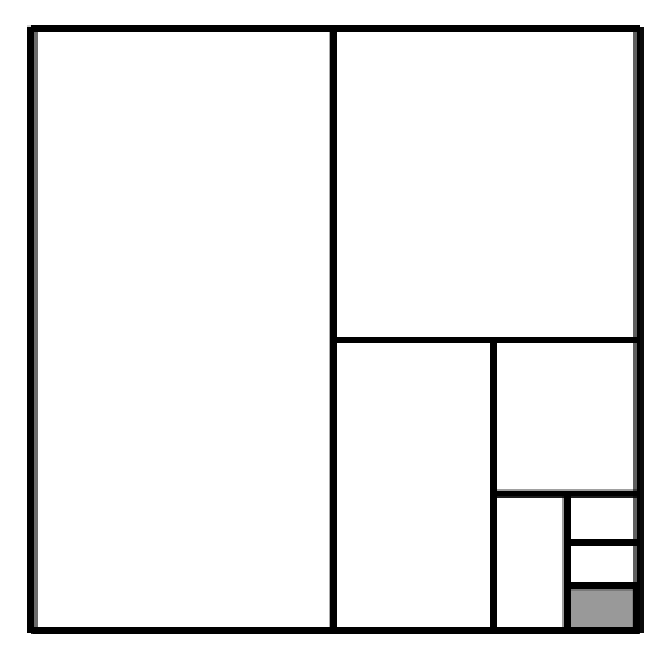
\includegraphics[scale=0.3]{carre_proportions.eps}
\end{center}
Which fraction corresponds with the shaded section?\\

a) $\frac{1}{96}$\\[2mm]
b) $\frac{1}{64}$\\[2mm]
c) $\frac{1}{16}$\\[2mm]
d) $\frac{1}{8}$\\

Answer: a)\\

Explanation:\\
In Russian manuscripts, the shaded section is described as "half of the half of the half of the half of the half of the third." In other words,
\begin{eqnarray*}
\frac{1}{2} \times \frac{1}{2} \times \frac{1}{2} \times \frac{1}{2} \times \frac{1}{2} \times \frac{1}{3} = \frac{1}{96}
\end{eqnarray*}
Thus, the answer is a).\\



3012-- Who used to use fractions like we do now in modern times?\\

a) Babylonians\\
b) Chinese\\
c) The men from Cro-Magnon\\
d) Martians\\

Answer: b)\\

Explanation:\\
In 100 B.C., the Chinese used fractions like we do for similar purposes: they avoided "improper" fractions, in other words, fractions formed by $\frac{7}{3}$. Instead, they wrote $2 \frac{1}{3}$. The correct answer is b).\\



3013-- The Chinese used the denominator method, commonly used to divide two fractions, for example, $\frac{2}{3} \div \frac{4}{5}$. The method states that in each fraction, the numerator and the denominator must be multiplied to the denominator of the other fraction:\\
\begin{eqnarray*}
\frac{2}{3} \ \div \ \frac{4}{5} \ = \ \frac{2\cdot5}{3\cdot5} \ \div \ \frac{3\cdot4}{3\cdot5} \ = \ \frac{10}{15} \ \div \ \frac{12}{15}.
\end{eqnarray*}
Since the two fractions are now above the same denominator, the problem can be resolved thru the simple division of whole numbers:
\begin{eqnarray*}
\frac{2}{3} \ \div \ \frac{4}{5} \ = \ \frac{10}{15} \ \div \ \frac{12}{15} \ = \ 10 \ \div \ 12 \ = \ \frac{5}{6}.
\end{eqnarray*}
By using this method, calculate $\frac{3}{4} \ \div \ \frac{9}{11}$.\\

Answer: $\frac{11}{12}$\\

Explanation:\\
\begin{eqnarray*}
\frac{3}{4} \ \div \ \frac{9}{11} \ &=& \ \frac{3\cdot11}{4\cdot11} \ \div \ \frac{4\cdot9}{4\cdot11}\\[2mm]
&=& \ \frac{33}{44} \ \div \ \frac{36}{44}\\[2mm]
&=& \ 33 \ \div \ 36\\[2mm]
&=& \ \frac{11}{12}
\end{eqnarray*}
Thus, the correct answer is $\frac{11}{12}$.\\



3014-- The reverse multiplication method requires inversing the divisor and multiplying it to the dividend. For example,
\begin{eqnarray*}
\frac{2}{3} \ \div \ \frac{4}{5} \ = \ \frac{2}{3} \ \times \ \frac{5}{4} \ = \ \frac{10}{12} \ = \ \frac{5}{6}.
\end{eqnarray*}
Around 850 A.D., who was the first to practice this method?\\

a) Apollonius\\
b) Rene Descartes\\
c) Mahavira\\
d) Multit Plie Kassion\\

Answer: c)\\

Explanation:\\
The reverse multipication method can only be used if in a fraction, one number is written above the other. Indian mathematicians were the first to write fractions in this way. More specifically, it was the Indian mathematician Mahavira who practiced the reverse multiplication method around 850 A.D. Thus, the correct answer is c).\\



3015-- The term "percent" or "percentage" is the name given to fractions whose denominator is 100. It was during the 15th and 16th centuries that this term was first used in a context other than that of pure mathematics. Which one?\\

a) Trade\\
b) Tax collecting\\
c) Medecine\\
d) Urbanization\\

Answer: a)\\

Explanation:\\
It was common in those days to calculate commercial interest rates by using percentage. This particular custom has remained in the business field even today. It is also one of the reasons why our monetary system is based on the dollar and the "cent". Thus, the correct answer is a).\\



3016-- Which one of these symbols has never been used to represent a percentage?\\

a) per 100\\[2mm]
b) $\frac{0}{0}$\\[2mm]
c) \%\\[2mm]
d) $\scriptstyle0/100$\\[2mm]

Answer: d)\\

Explanation:\\
\begin{center}
\begin{tabular}{|c|c|}
\multicolumn{2}{c}{\bf \ Evolution of the percent sign}\\[2mm] \hline
{\bf Year} & {\bf Symbol} \\[1mm] \hline \hline
1425 & `` \emph{percent} '' \ \ by hand \\[1mm] \hline
around 1650 & `` for $\frac{0}{0}$ '' \\[1mm] \hline
a few years later & `` $\frac{0}{0}$ '' \\[1mm] \hline
today & `` \% '' \\[1mm] \hline
\multicolumn{2}{c}{}
\end{tabular}
\end{center}
The symbol that has never existed is `` $\scriptstyle0/100$ ''. The correct answer is d).\\



3017-- In which century did number writing in decimal notation (for example 0.25) become popular?\\

a) 3rd century\\
b) 16th century\\
c) 17th century\\
d) 21st century\\

Answer: b)\\

Explanation:\\
It was in 1585, in a book by Belgian mathematician, Simon Stevin, that fraction writing in decimal numbers was shown to be the most simple form of writing. For Stevin, the decimal number $0.333$ is a good estimation of the fraction $\frac{1}{3}$. Today we know that $\frac{1}{3} = 0,\overline3$, in other words, that there is an infinite quantity of 3 after the decimal point. Thus, the correct answer is b).\\
\begin{center}
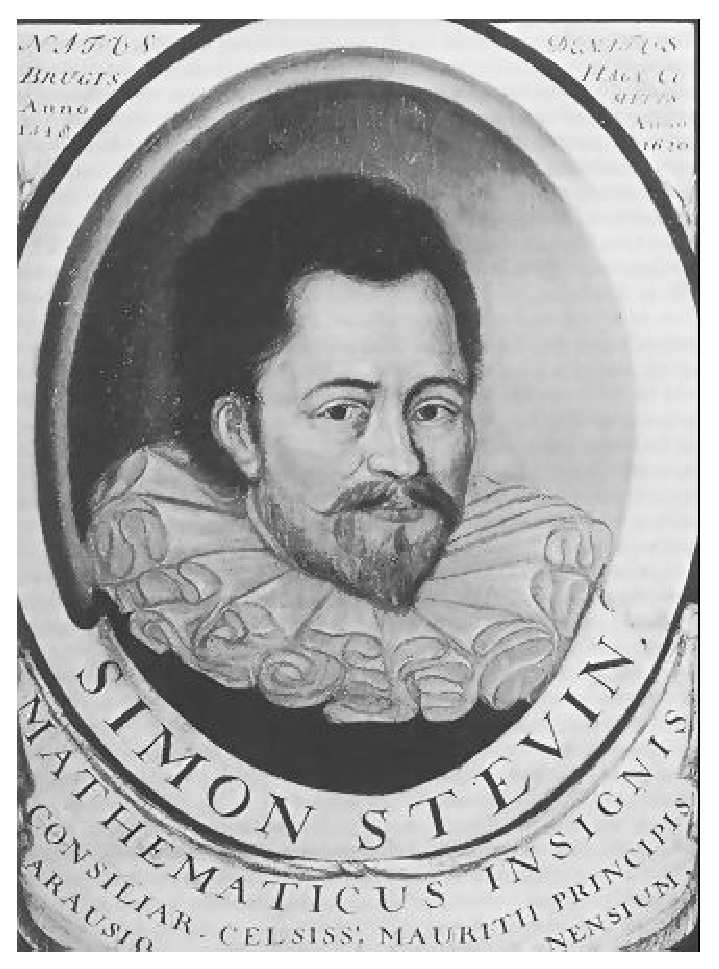
\includegraphics[scale=0.25]{stevin.eps}\\
\emph{{\small Simon Stevin}}\\
\href{http://fr.wikipedia.org/wiki/Simon Stevin}{fr.wikipedia.org/wiki/Simon Stevin}[5mm]
\end{center}



3018-- In what year was the first arithmetic book printed in North America using a comma to separate the integral part of a mixed number from its fractional part?\\

a) 500 B.C.\\
b) 1300\\
c) 1729\\
d) 1919\\

Answer: c)\\

Explanation:\\
The first arithmetic book using a comma to separate the integral part from the fractional part of a number was printed in North America in 1729. Soon thereafter, some books began using a decimal point in place of a comma. Today, the comma is used in French and the decimal point in English. Thus, the correct answer is c).\\



3019-- What Flemish (Belgian) mathematician was the first to consider real numbers ($\mathbb{R}$) to be points on a straight line?\\

a) Gerardus Mercator\\
b) Nicolaus Copernicus\\
c) Gesuit Bellje\\
d) Simon Stevin\\

Answer: d)\\

%{\bf\textsf{animation : chaque description du math\'ematicien appara\^it avec son image : le petit bonhomme pourrait les pousser ou tirer, sur son skateboard}}\\
Explanation:\\
Gerardus Mercator was a mathematician/geographer who recorded the first image of Earth on paper (in other words, he drew the first-ever map).
\begin{center}
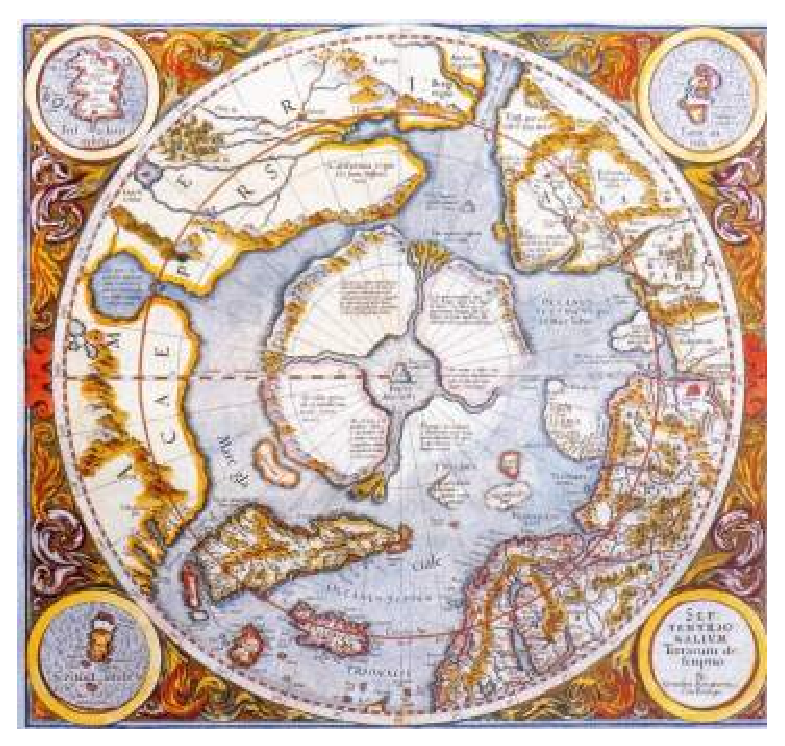
\includegraphics[scale=0.3]{carte.eps}\\
\emph{{\small carte du P\^ole Nord par Gerardus Mercator (fin du 16\ieme{} si\`ecle)}}\\
\href{http://www.transpolair.com/images/cart161.jpg}{www.transpolair.com/images/cart161.jpg}
\end{center}
Nicolaus Copernicus, Polish doctor and astronomer, drew the first heliocentric model of the solar system (heliocentric means to which the sun is the center). In other words, he had imagined the solar system as we know it today.
\begin{center}
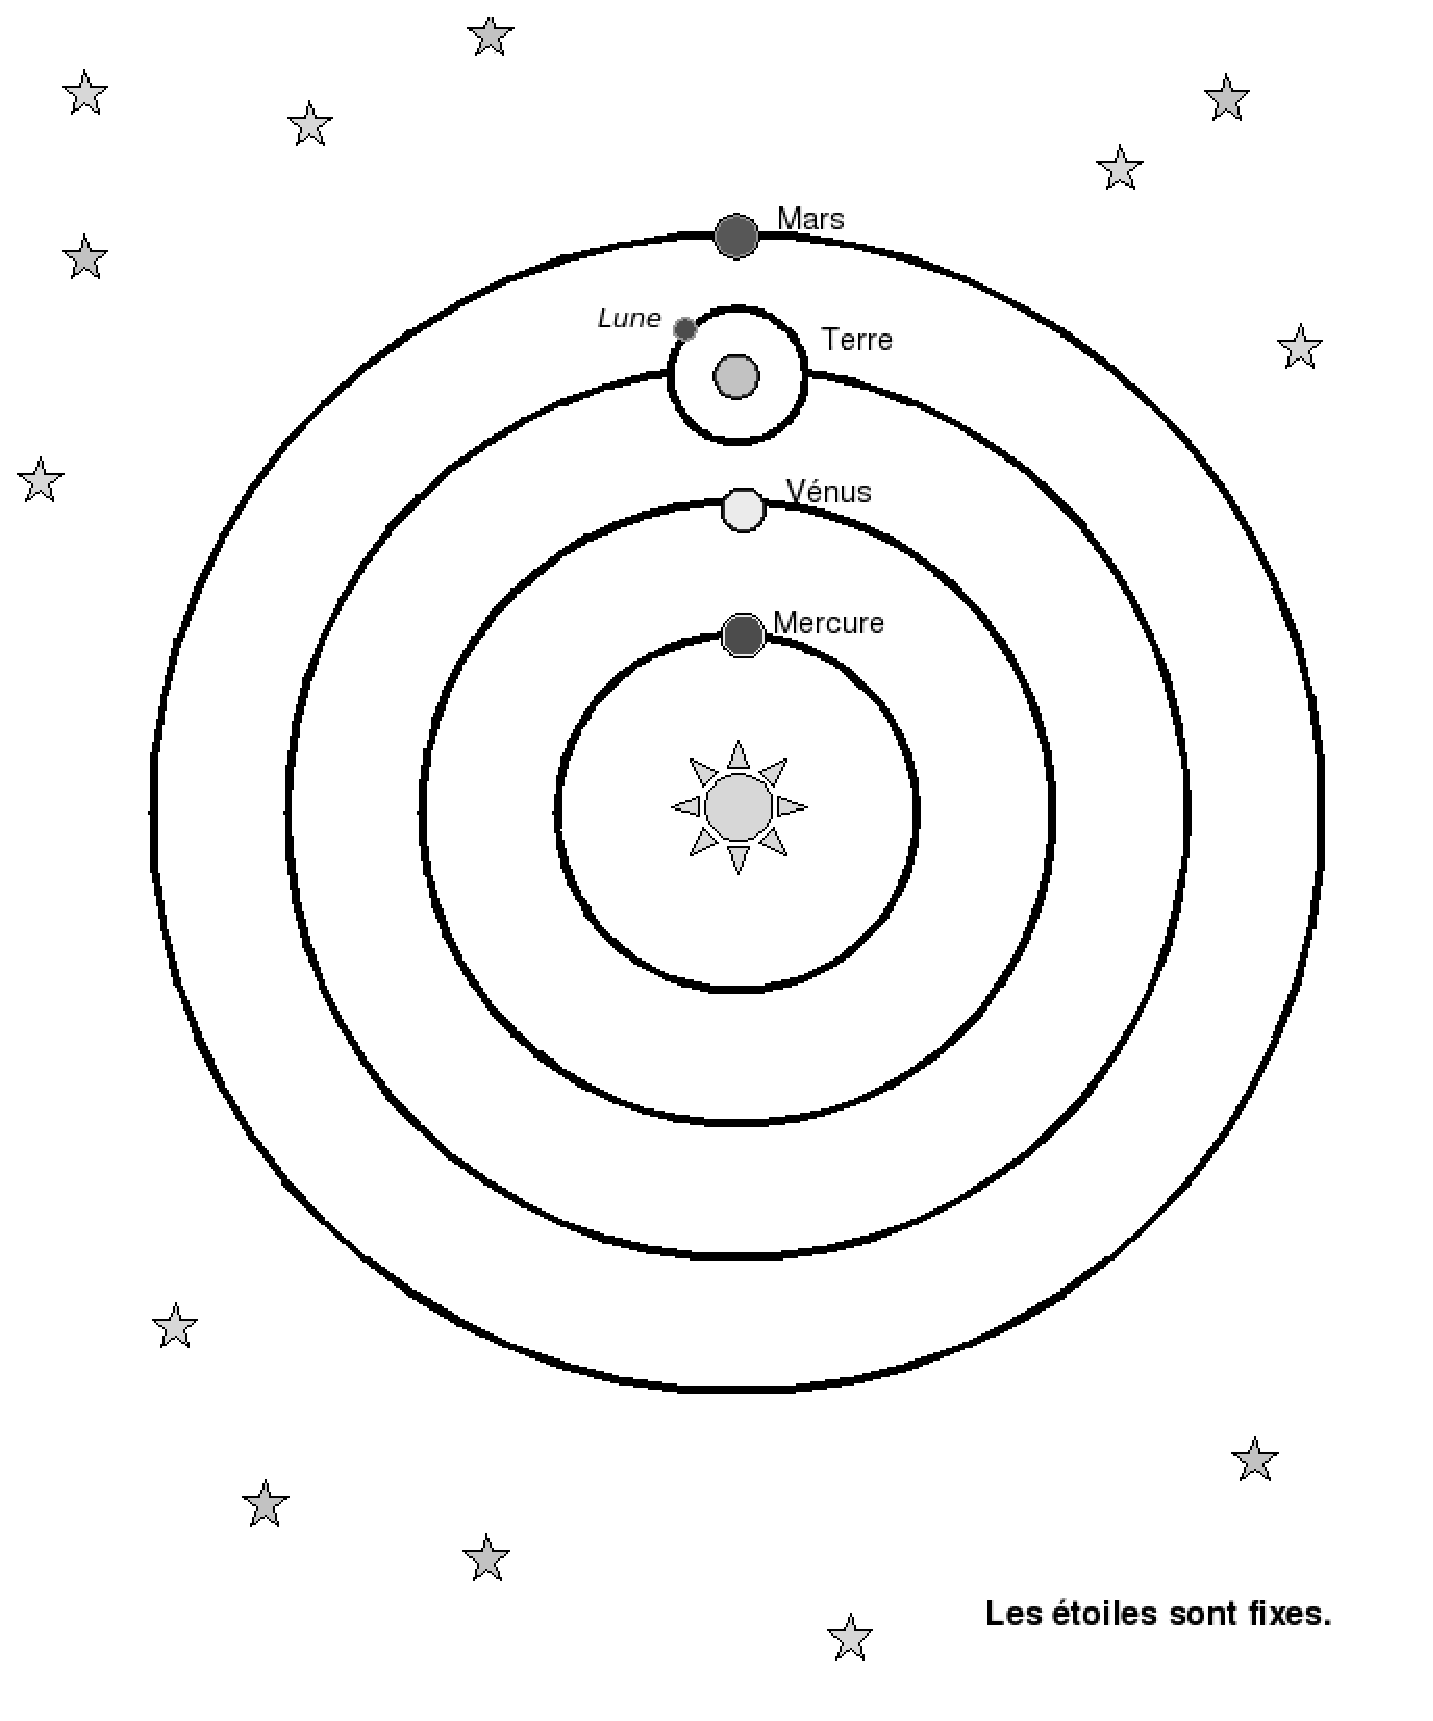
\includegraphics[scale=0.25]{heliocentrique.eps}\\
\emph{{\small syst\`eme copernicien, h\'eliocentrique}}
\end{center}

Lastly, Simon Stevin was the first mathematician to consider real numbers to be points on a straight line. Thus, the correct answer is d).\\
\begin{center}
\includegraphics[scale=0.25]{droitereelle.eps} {\large$\mathbb{R}$}\\
\emph{{\small droite r\'eelle}}
\end{center}



3020-- Negative numbers have existed since 1500 B.C.?\\
True or False?\\

Answer: False\\

Explanation:\\
At the time that Christopher Columbus discovered America, negative numbers didn't exist.  It wasn't until 200 years later that they were accepted into the number family. Thus, the correct answer is: False.\\
In the beginning, numbers were used mainly to count objects. When the number 0 became widely accepted, it was considered to be the smallest of all numbers. After all, what could be smaller than nothing at all?\\ (Still, mathematicians knew that such numbers existed, but in their problems, like for example, find the solution of $4x + 20 = 4$, they simply rejected any negative answer (there were no solutions to these equations in those days, even if $x = -4$ was a solution)).\\



3021-- Who was the first Indian mathematician to work with negative "quantities"? (not numbers, but quantities)\\

a) Brahmagupta\\
b) Tuhaf Detz\\
c) Carl Friedrich Gauss\\
d) Pythagoras\\

Answer: a)\\

Explanation:\\
Brahmagupta {\small(598-668)}, an Indian mathematician worked with assets (positive quantities) and debts (negative quantities). He even created rules to add, subtract, multiply and divide these assets and debts. Thus, the correct answer is a).\\



%{\bf\textsf{animation : petit bonhomme avec tout plein de points d'interrogation autour de sa t\^ete}}\\
3022-- {If $-1$ is smaller but not equal to 1, then $\frac{-1}{1} = \frac{1}{-1}$ cannot be valid, for the smallest number over the largest cannot be equal to the largest number over the smallest. For example: $1 < 3 \ \textrm{et} \ \frac{1}{3} \neq \frac{3}{1}$.}\\[2mm]
Who was the 17th century mathematician to first raise this question?\\

a) Antoine Arnauld\\
b) Euclid\\
c) Omar Khayyam\\
d) Sim\'eon Denis Poisson\\

Answer: a)\\

Explanation:\\
Even after the acceptance of negative numbers in the number family, 17th century mathematicians had trouble putting them in the right order. How could $-1$ be smaller than 1, while their ratios $\frac{-1}{1}$ et $\frac{1}{-1}$ are equal? Antoine Arnauld {\small (1612-1694)} was the first to raise this question. Thus, the correct answer is a).

\begin{center}
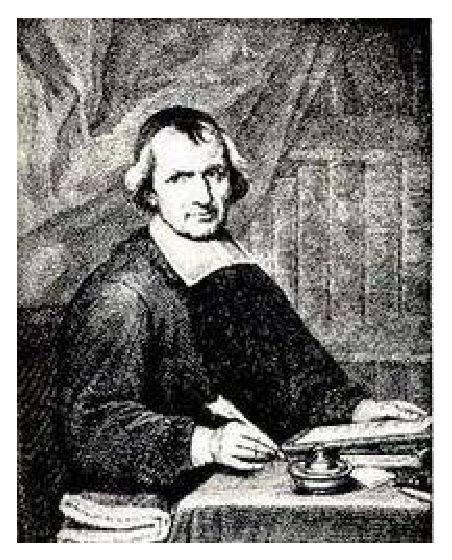
\includegraphics[scale=0.5]{Antoine_Arnauld.eps}\\
\emph{{\small Antoine Arnauld}}\\
\href{http://fr.wikipedia.org/wiki/Antoine Arnauld}{fr.wikipedia.org/wiki/Antoine Arnauld}\\[5mm]
\end{center}



3023-- Which mathematician believed (even if we know now that it is not true) that negative numbers were larger than infinity ($\infty$)?\\

a) Georges Cantor\\
b) Henri Navier\\
c) John Wallis\\
d) Joseph Fourier\\

Answer: c)\\

Explanation:\\
In the book `` \emph{Arithmetica Infinitorum} '' \ by John Wallis, he states that `` \emph{numbers inferior to 0 are larger than infinity} ''. \ The correct answer is c), John Wallis.
\begin{center}
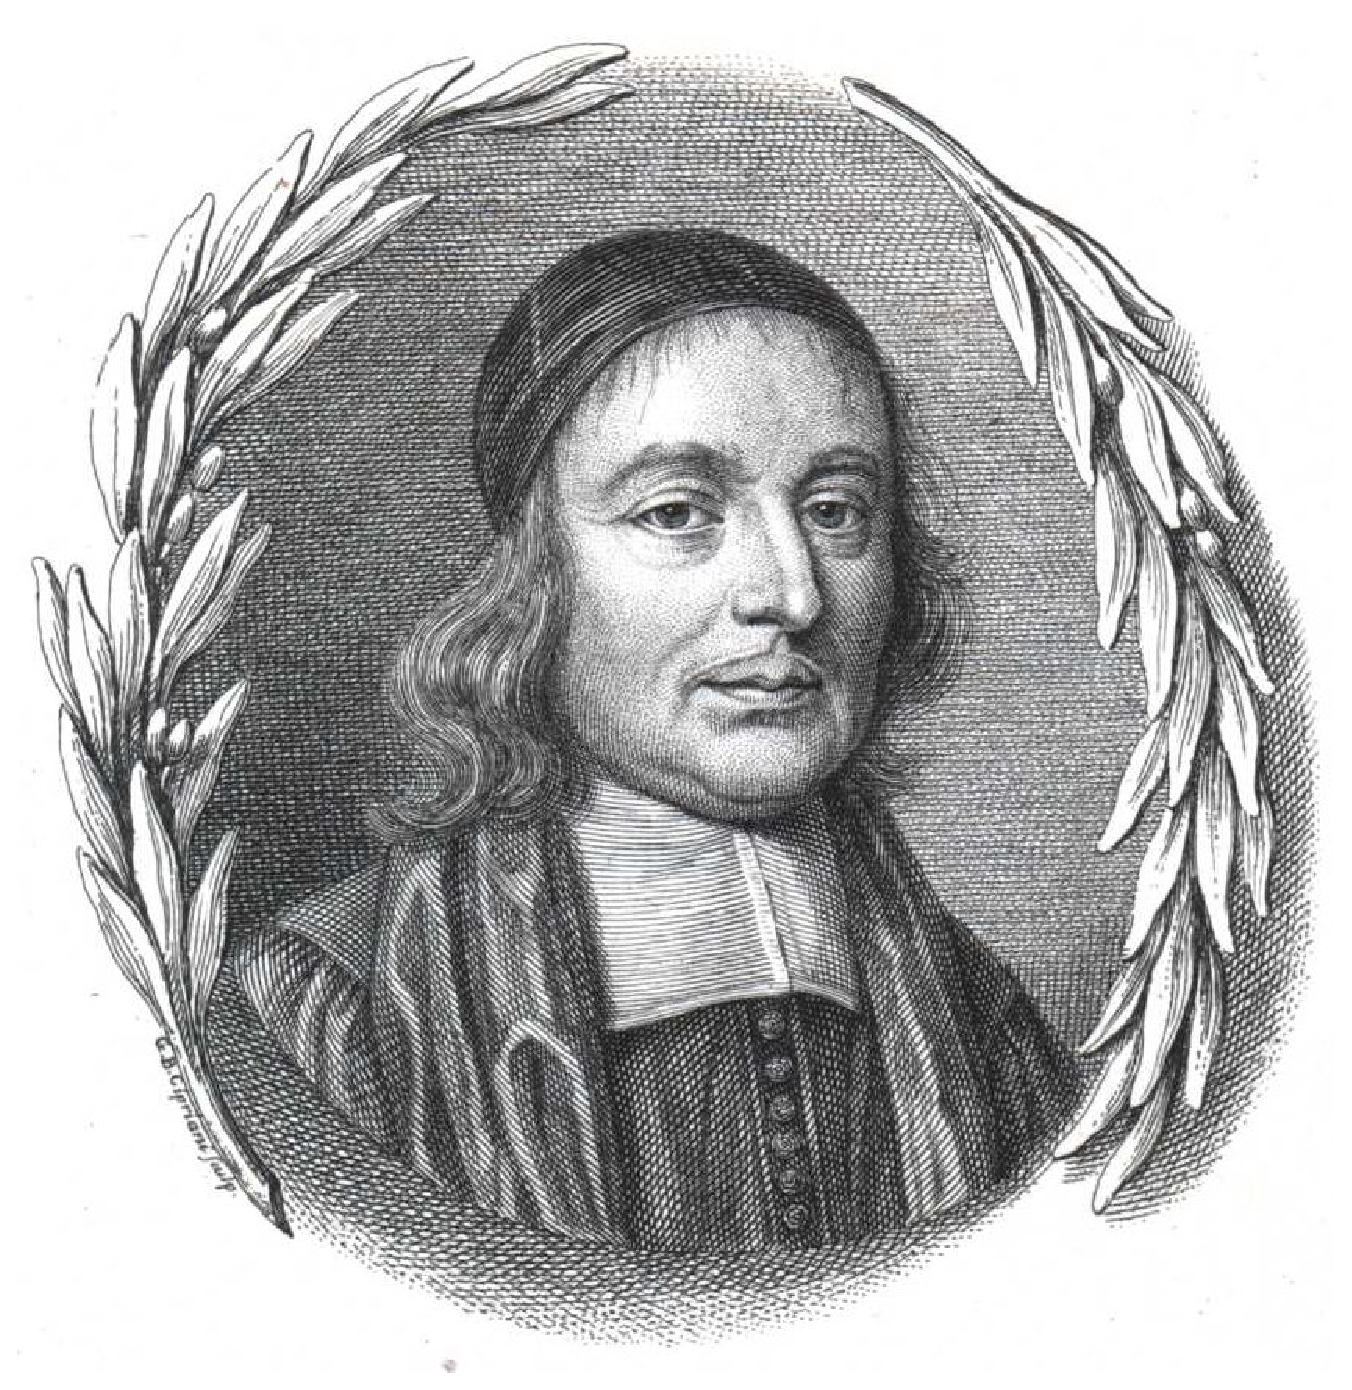
\includegraphics[scale=0.2]{John_Wallis.eps}\\
\emph{{\small John Wallis}}\\
\href{http://fr.wikipedia.org/wiki/John Wallis}{fr.wikipedia.org/wiki/John Wallis}
\end{center}

Explaining his reasoning: \emph{Since \ $\frac{3}{0} = \infty$, a denominator smaller than $0$ chosen in another fraction, makes the new fraction larger than $\frac{3}{0}$ (for example, since $1 < 2$, then $3 = \frac{3}{1} > \frac{3}{2} = 1,5$). In this way, since $-1 < 0$, then $\frac{3}{-1} > \frac{3}{0} = \infty$. We know now that even if $-1 < 0$, $-3 = \frac{3}{-1} < \frac{3}{0} = \infty$.}\\



3024-- Which well-known English physicist and mathematician said the following: `` \emph{Quantities are positive and larger than nothing or negative and smaller than nothing.}''?\\

a) Georges Adams\\
b) Isaac Newton\\
c) Johnny Test\\
d) Michel Rolle\\

Answer: b)\\

Explanation:\\
Contrary to common belief, Isaac Newton did not only work in the physics field. In 1707, in a book that he wrote `` \emph{Universal Arithmetick} '', he illustrated that positive quantities are larger than zero and negative quantities are smaller than zero. Since Newton was a great scientist in his era, his idea was taken very seriously. Thus, the correct answer is b).\\

\begin{center}
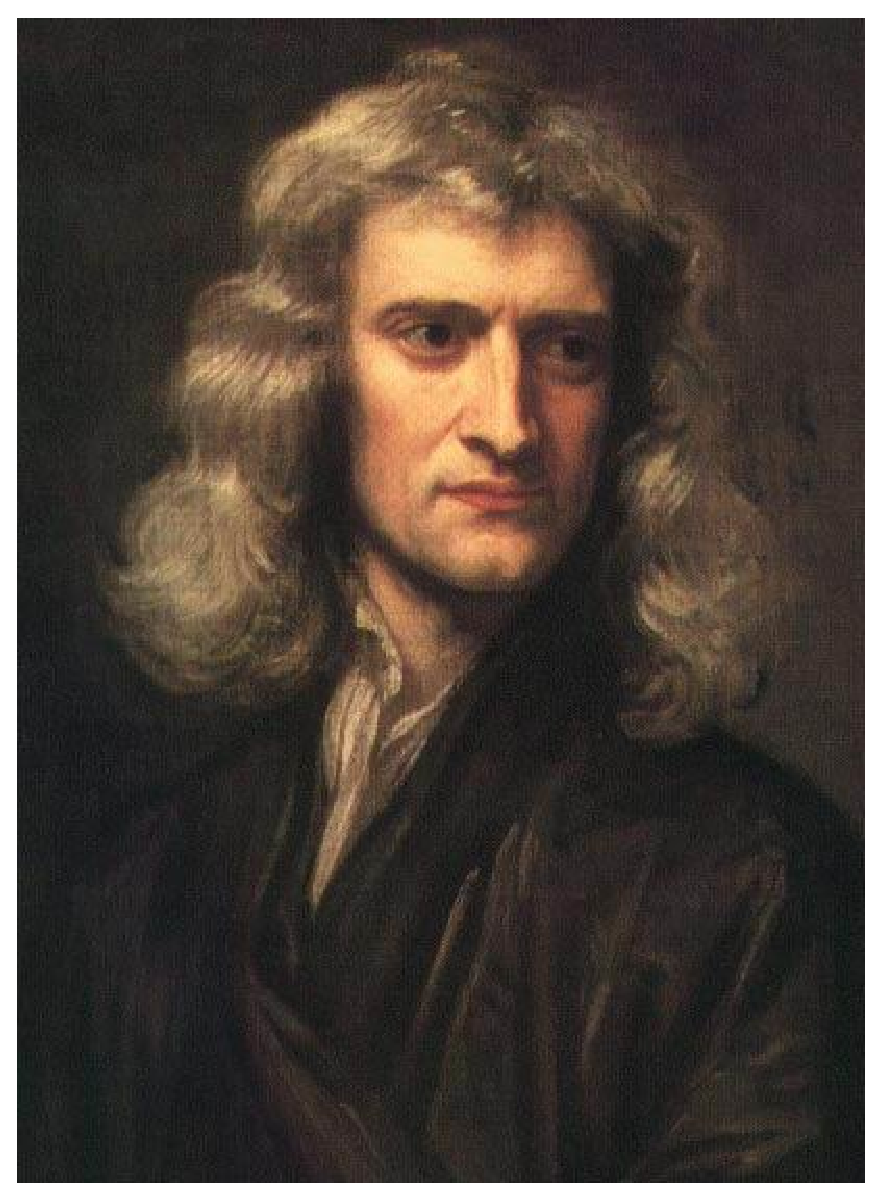
\includegraphics[scale=0.2]{IsaacNewton.eps}\\
\emph{{\small Isaac Newton}}\\
\href{http://fr.wikipedia.org/wiki/Isaac Newton}{fr.wikipedia.org/wiki/Isaac Newton}\\[5mm]
\end{center}



3025-- Which 18th century Swiss mathematician said: `` \emph{Negative numbers can be considered as debts because positive numbers represent real possessions. It can be said that negative numbers are less than nothing. In this manner, when a man possesses nothing and he owes 50 crowns, he must have 50 crowns less than nothing. If someone gives him a gift of 50 crowns to pay his debts, he will only be at zero, but he will be richer than before}'' ?\\[2mm]

a) Fran\c cois Vi\`ete\\
b) Jean-Marie De Koninck\\
c) Leonhard Euler\\
d) Pierre Fatou\\

Answer: c)\\

Explanation:\\
In 1770, `` \emph{Elements of Algebra} '', Leonhard Euler recaptured, in one way or another, the same ideas that the Chinese had come up with 17 centuries earlier, in other words,  he considered positive numbers as assets and negative numbers as debts. The correct answer is c).\\

\begin{center}
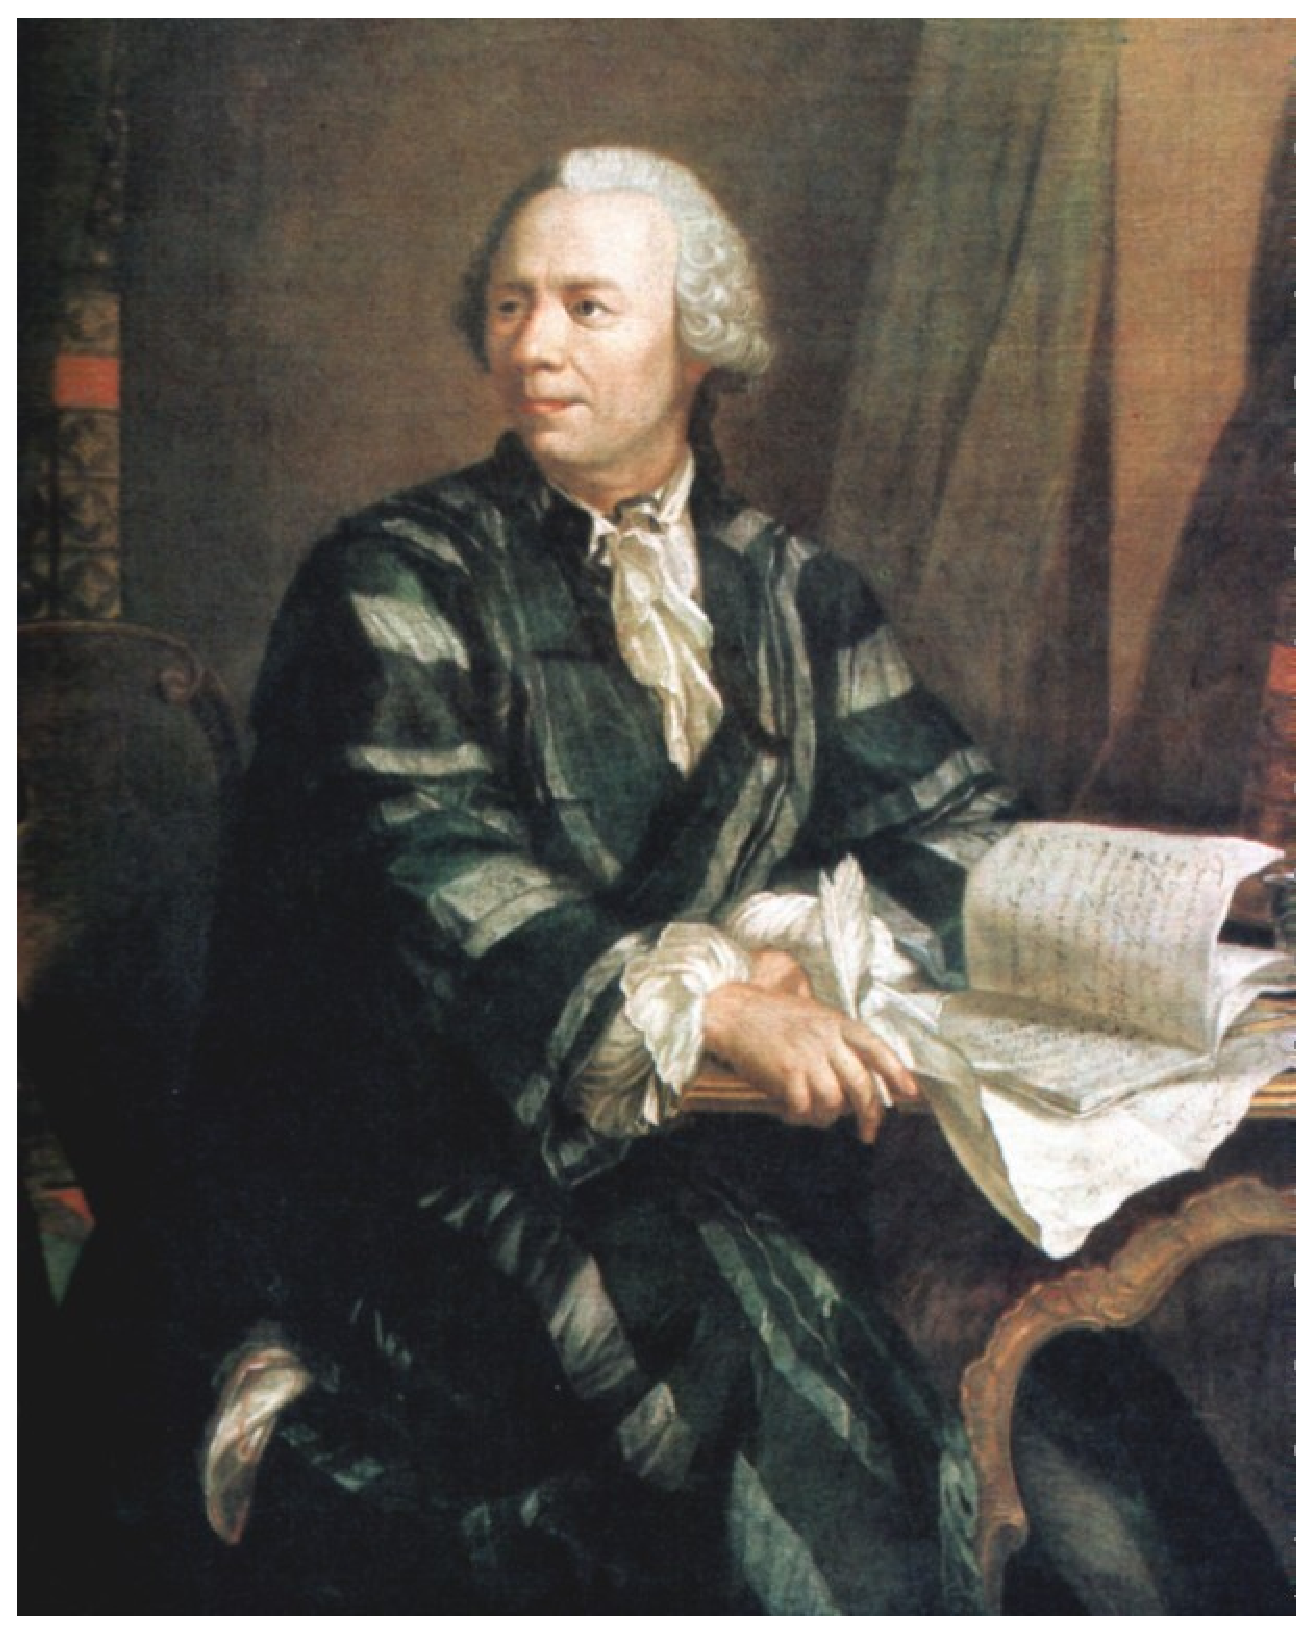
\includegraphics[scale=0.15]{Euler.eps}\\
\emph{{\small Leonhard Euler}}\\
\href{http://fr.wikipedia.org/wiki/Leonhard Euler}{fr.wikipedia.org/wiki/Leonhard Euler}\\[5mm]
\end{center}



3026-- \'Evariste Galois was a French mathematician born in Paris, in 1811. He was considered as the inventor of the Group Theory. When did he pass away? (Tell yourself that if we are asking the question, there certainly must be a reason\dots)\\

\begin{center}
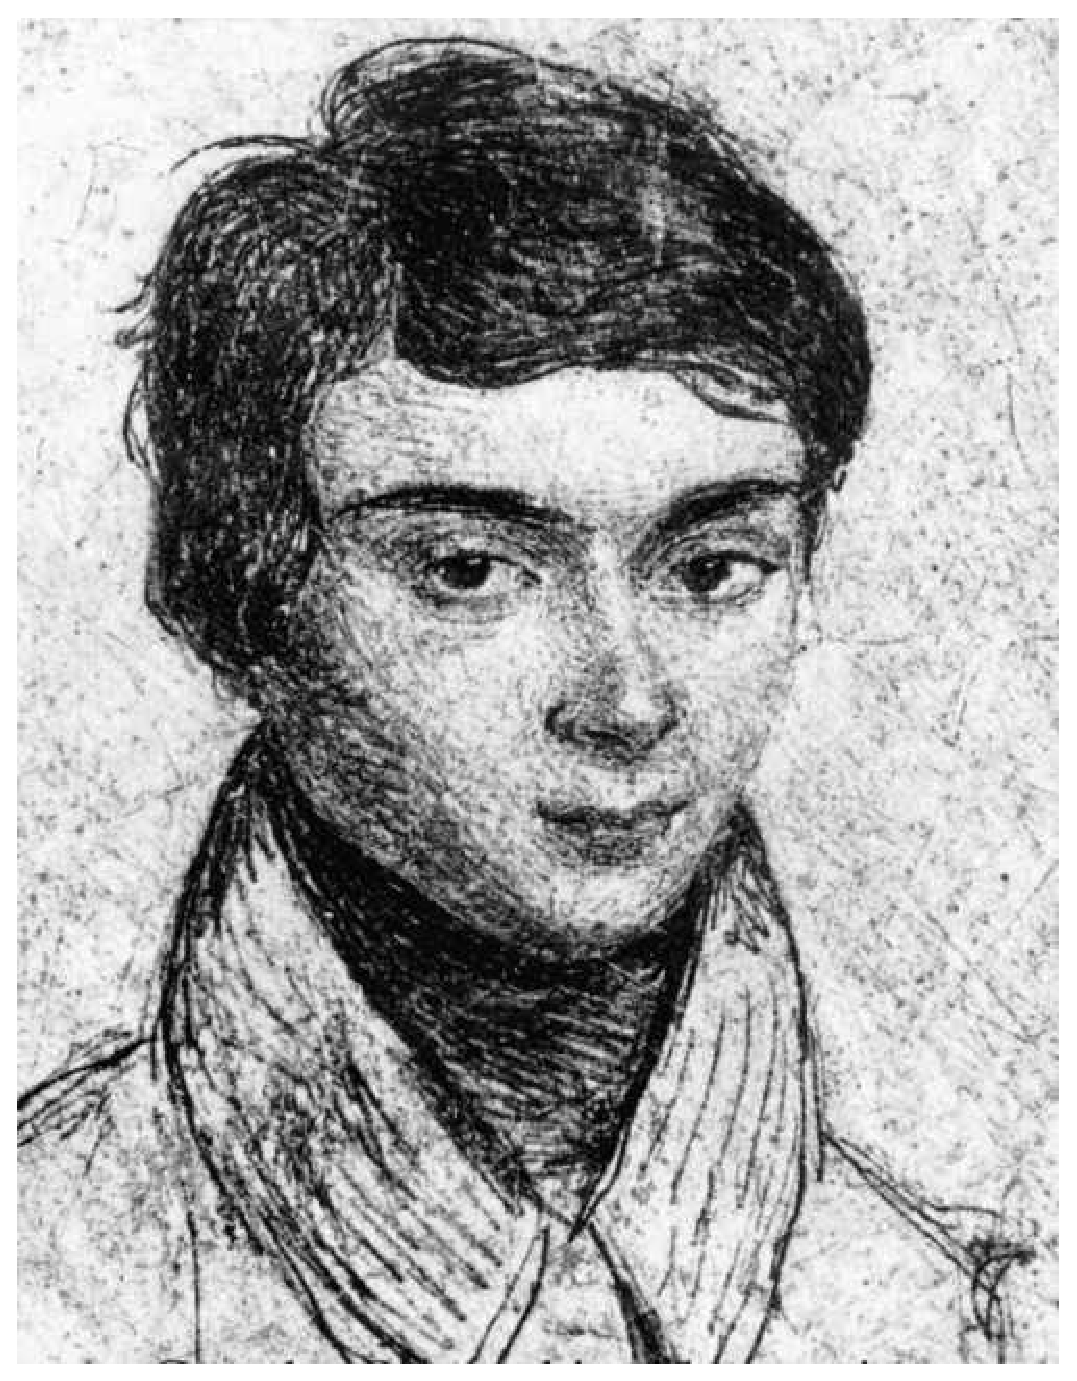
\includegraphics[scale=0.15]{Evariste_galois.eps}\\
\emph{{\small \'Evariste Galois}}\\
\href{http://fr.wikipedia.org/wiki/Evariste Galois}{fr.wikipedia.org/wiki/Evariste Galois}
\end{center}

a) 1832\\
b) 1855\\
c) 1870\\
d) 1911\\

Answer: a)\\

%{\bf \textsf{animation : petit bonhomme pourrait faire de l'escrime}}\\
Answer:\\
Galois died in 1832 at the age of 20. He lost his life in a duel defending a woman's honor. Thus, the correct answer is a).\\



3027-- According to the legend, how did King Henry I defend his idea that a yard would be 36 inches long?\\

a) That same very day, he hunted and trapped a small animal that was 36 inches long.\\
b) He had very large feet and the total length of his two feet was 36 inches.\\
c) When he took a large step in front of him, the distance between the end of his toes of his front foot and the heel of his back foot was 36 inches.\\
d) When he reached his arms out straight in front of him, there was a distance of 36 inches between the end of his nose and his thumbs.\\

Answer: d)\\

%{\bf \textsf{animation : petit bonhomme, d\'eguis\'e en roi, qui mesure la distance de son nez \`a ses pouces}}\\
Explanation:\\
One day, to end all confusion on what was the exact length of a yard, King Henry I decided that it would be the length equal to the distance between the end of his nose and his thumbs. He held his arms out straight in front of him, and this distance was measured: `` \emph{36 thumbs!} ''. It was in that moment that a yard was officially declared 36 inches (thumbs) long. The correct answer is d).\\



3028-- Meters were created in reference to 1/10,000,000 of the length of the Earth's arc at sea-level between the North Pole and the South Pole.\\
True or False?\\

Answer: False\\

Explanation:\\
The French Academy of Science defined meters as 1/10,000,000 the length of the Earth's arc between the North Pole and the \emph{\underline{Equator}}, and not the South Pole. The answer is: False. The Earth's circonference measures approximately $40\,000$ kilometers long. The quarter of this circonference, which is in fact the arc between the North Pole and the Equator, is about $10,000$ kilometers long. 1/10,000,000 of $10\,000$ kilometers is equal to 0.001 kilometer, or one meter.
\begin{eqnarray*}
10\,000\,\text{km} \div 10\,000 000 &=& 0,001\,\text{km}\\
&=& 0,001\,\text{km} \times \frac{1\,000\,\text{m}}{1\,\text{km}}\\
&=& 1\,\text{m}\\
\end{eqnarray*}
\begin{center}
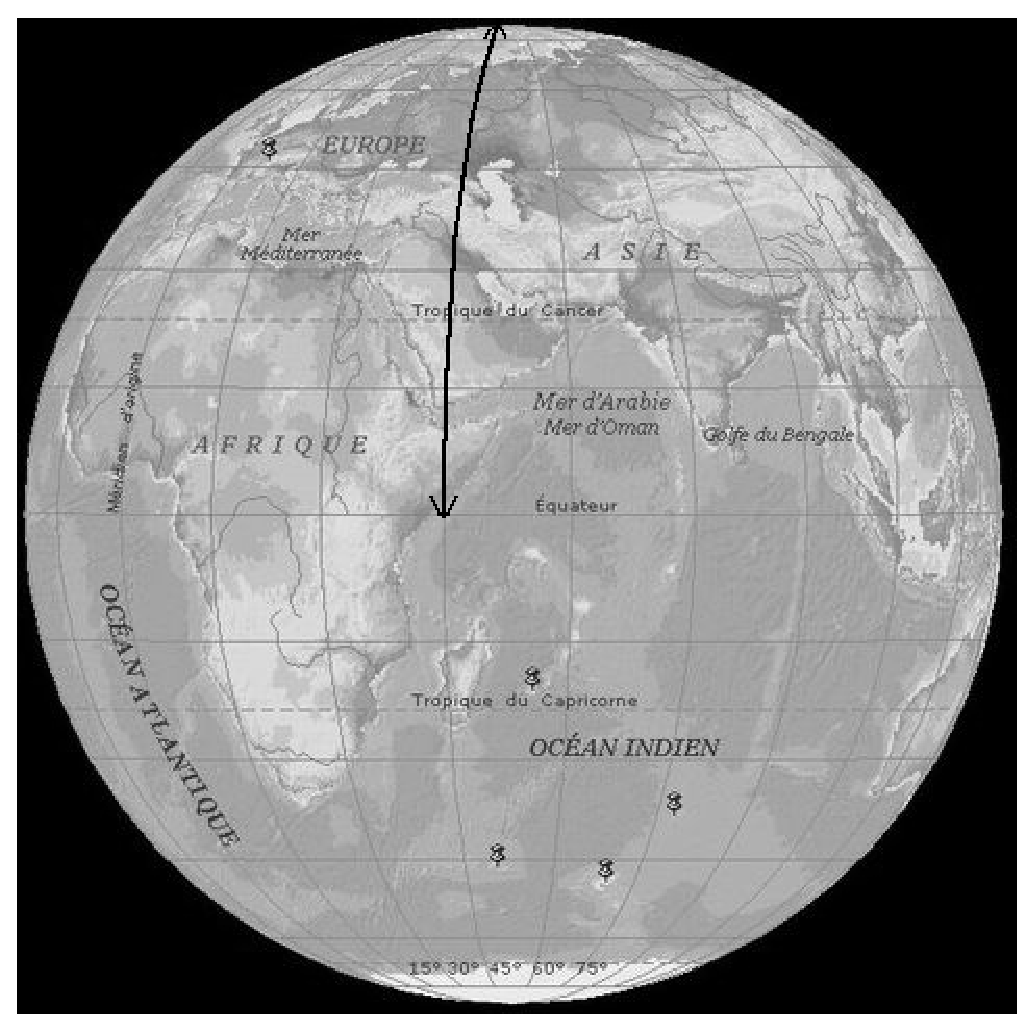
\includegraphics[scale=0.25]{terre.eps}\\
\href{http://collegevanoise.fr/images/ign/maurice.jpg}{collegevanoise.fr/images/ign/maurice.jpg}\\[5mm]
\end{center}



3029-- Units of measure smaller than a meter have a Latin prefix and units of measure larger than a meter have a Greek prefix.\\
True or False?\\

Answer: True\\

Explanation:\\
The fact that units of measure smaller or larger than a meter be in powers of 10, makes the metric system easier to understand.\\

\begin{center}
\begin{tabular}{|l|c|l|} \hline
{\it Nom} & {\it Symbol} & {\it Quantity in digits}  \\ \hline \hline
\textbf{giga}meter & Gm & $1 \, 000 \, 000 \, 000$\\ \hline
\textbf{mega}meter & Mm & $1 \, 000 \, 000$\\ \hline
\textbf{kilo}meter & km & $1 \, 000$\\ \hline
\textbf{hecto}meter & hm & $100$\\ \hline
\textbf{deca}meter & dam & $10$\\ \hline
meter & m & $1$\\ \hline
\textbf{deci}meter & dm & $0,1$\\ \hline
\textbf{centi}meter & cm & $0,01$\\ \hline
\textbf{milli}meter & mm & $0,001$\\ \hline
\textbf{micro}meter & $\mu$m & $0,000 \, 001$\\ \hline
\textbf{nano}meter & nm & $0,000 \, 000 \, 001$\\ \hline
\multicolumn{3}{c}{}\\
\end{tabular}
\end{center}

The prefixes for units smaller than a meter (deci-, centi-, milli-, \dots) are Latin. The prefixes for units larger than a meter (deca-, hecto-, kilo-, \dots) are Greek. The correct answer is: True.\\



3030-- A kilogram is defined as being the amount of pure water contained in a meter-long cube held on its side.\\
True or False?\\
\begin{center}
\includegraphics[scale=0.3]{cube.eps}
\end{center}

Answer: False\\

%{\bf \textsf{animation : petit bonhomme pourrait intervenir ici $\rightarrow$ regarder ou lui-m\^eme remplir les cubes d'eau?}}\\
Explanation:\\
A kilogram is defined as being the amount of pure water contained in a \emph{\underline{decimeter}}-long cube held on its side and not a meter-long cube. The correct answer is: False. This measurement is equal to one liter ($1\,\text{dm}^{3}\,=\,1\,\text{l}$).\\

\begin{center}
\includegraphics[scale=0.3]{cubedm.eps}
\end{center}



3031-- Which angle measurement was invented in order to calculate the length of the Earth's arc?\\

a) degree\\
b) grade\\
c) rad\\
d) minute\\

Answer: b)\\

Explanation:\\
In attempting to calculate the length of the Earth's arc, researchers hired by the French Academy of Science decided to invent an angle measurement that would use powers of 10, in the same manner as the metric system. They then established the measurement for a right angle equal to 100 grades (90$^\circ$ = 100 gr). The correct answer is b).\\



3032-- To which German mathematician do we owe the definition of a function in terms of set pairs, in other words $y = f(x)$?\\

a) Bjornen Atinephortifhive\\
b) Georg Cantor\\
c) Pythagoras\\
d) William Brouncker\\

Answer: b)\\

Explanation:\\
Georg Cantor's work is at the origin of the Set Theory. He defined a function as being a set of pairs. As Cantor explains, a function can be drawn in Cartesian, in other words, according to $x$ and $y$. For example, $y = f(x) = x^{3} + x^{2} + x$.
%Cela a permis \`a Cantor de d\'efinir la fonction bijective ou bijection (si on prend un \'el\'ement $y$ dans l'ensemble d'arriv\'ee (image ou codomaine), alors il existe un et un seul \'el\'ement $x$ dans l'ensemble de d\'epart (domaine) qui est une solution de la fonction $y = f(x)$.
\begin{center}
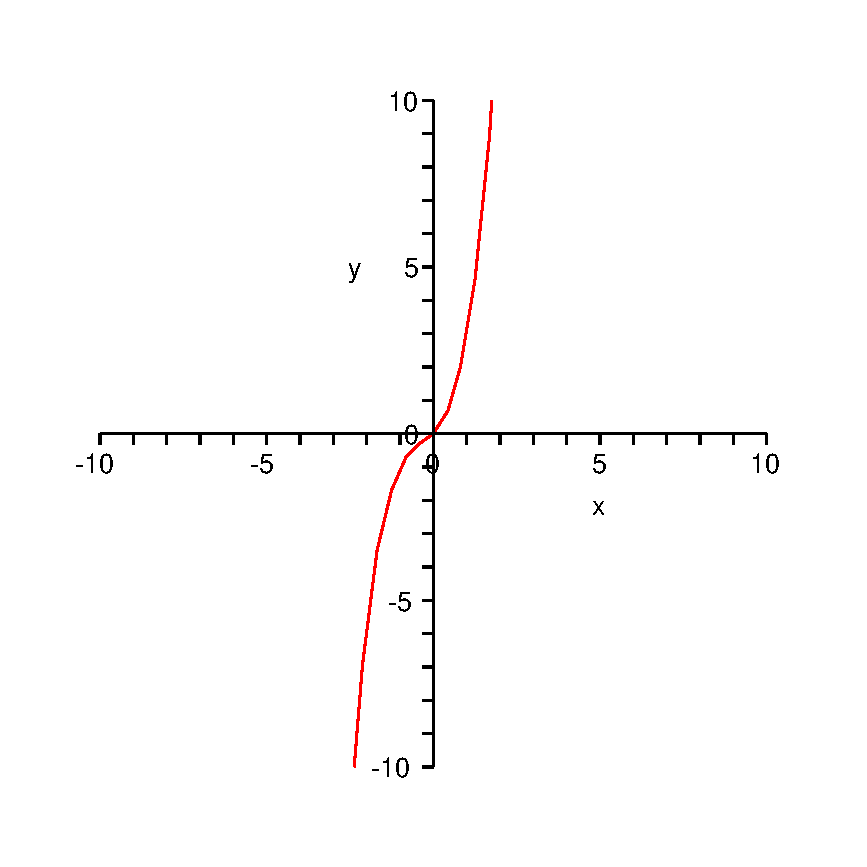
\includegraphics[scale=0.5]{fonction.eps}\\
$f(x) = x^{3} + x^{2} + x$\\
\end{center}
Thus, the answer is d).
\begin{center}
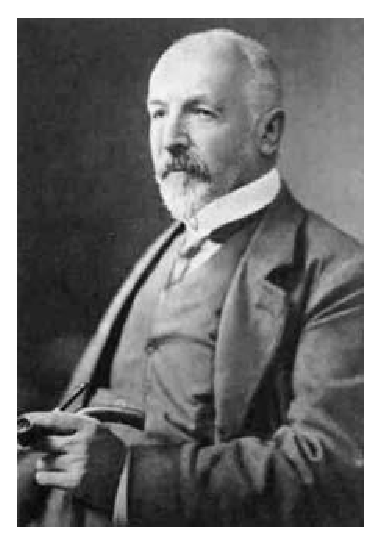
\includegraphics[scale=0.5]{Georg_Cantor.eps}\\
\emph{{\small Georg Cantor}}\\
\href{http://fr.wikipedia.org/wiki/Georg Cantor}{fr.wikipedia.org/wiki/Georg Cantor}\\[5mm]
\end{center}



%{\bf \textsf{animation : bonhomme d\'eguis\'e en Einstein qui regarde le mercure du thermom\`etre monter et descendre}}\\
3033-- In 1593, what mathematician invented the thermometer?\\

a) Archimedes of Syracuse\\
b) Galileo Galilei\\
c) Hidinit Hinventnuttin\\
d) Leonardo of Pisa (or Fibonacci)\\

Answer: b)\\

Explanation:\\
Archimedes of Syracuse's most well-known invention is the Archimedes screw. Leonardo of Pisa found the Fibonacci numbers $(1,1,2,3,5,8,13, \dots)$; so it can be said that he invented the follow-up to Fibonacci's numbers. Galileo Galilei assembled the first device allowing one to compare different levels of hot and cold. Thus, the correct answer is b)\\

\begin{center}
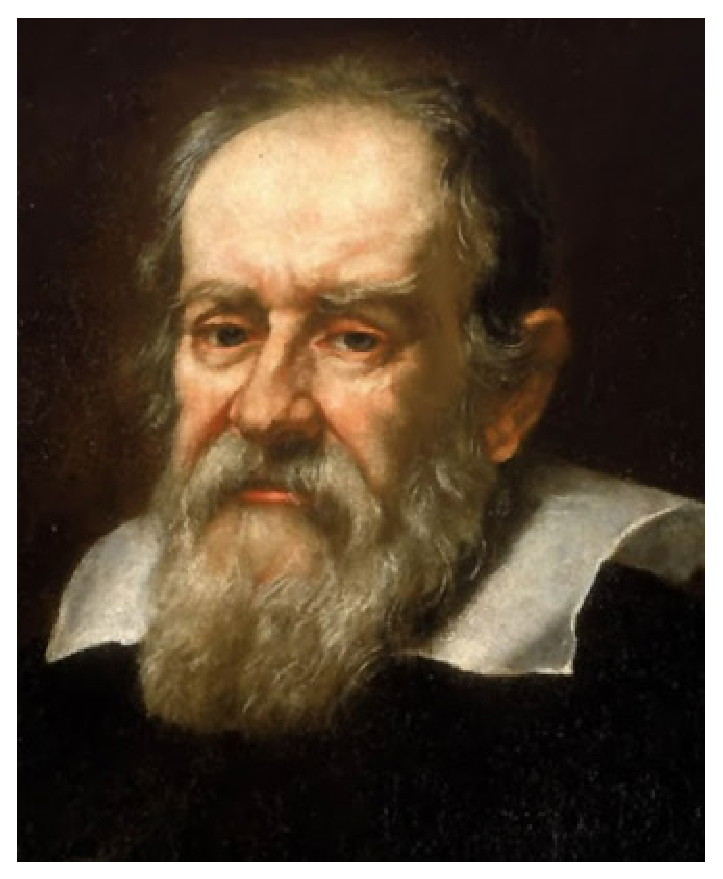
\includegraphics[scale=0.25]{Galilee.eps}\\
\emph{{\small Galileo Galilei}}\\
\href{http://fr.wikipedia.org/wiki/Galileo Galilei}{http://fr.wikipedia.org/wiki/Galileo Galilei}\\[5mm]
\end{center}



3034-- Christoff Rudolff composed a treaty, `` \emph{Das Coss} '', for `` \emph{the thing} '' \ in the meaning of the unknown of an algebraic equation. In 1525, what symbol did this German mathematician invent?\\

a) Empty set:\ \ $\varnothing$\\
b) Infinity:\ \ $\infty$\\
c) Natural set:\ \ $\mathbb{N}$\\
d) Square root:\ \ $\surd$\\

Answer: d)\\

Explanation:\\
The resolution of quadratic equations brings into play the notion of square roots. At that time, people needed some sort of notation to express this mathematic operation. Christoff Rudolff studied the resolution of algebraic equations. He used and invented notations as concise as possible, for instance the square root sign($\surd$). Thus, the correct answer is d). These days, the same sign is used the only difference being the bar above ($\sqrt{ \ \ }$).\\



%{\bf \textsf{animation : petit bonhhomme d\'eguis\'e en Harry Potter et qui vole sur son balai}}\\
3035-- Who developped a method to estimate the square root of any given number at the end of the 1st century?\\

a) Harry Potter\\
b) Heron of Alexandria\\
c) Jerome Cardan\\
d) Pierre-Simon Laplace\\

Answer: b)\\

Explanation:\\
Apart from Heron's formula used to calculate the area of any given triangle, Heron of Alexandria created a formula that estimated the square root of any given number. Thus, the correct answer is b).\\


% pas de niveau secondaire
%3036-- Quel concept math\'ematique a \'et\'e d\'efini par Augustin-Louis Cauchy, un math\'ematicien fran\c cais du 18\ieme si\`ecle et red\'efini plus tard par Eduard Heine, un math\'ematicien allemand du 19\ieme{} si\`ecle? (Heine trouvait que la d\'efinition de Cauchy n'\'etait pas assez claire et qu'elle pouvait \^etre plus pr\'ecise.)\\

%a) continuit\'e d'une fonction\\
%b) domaine d'une fonction\\
%c) fonction cosinus\\
%d) fonction sinus\\

%R\'eponse : a)\\

%R\'etoaction :\\
%Cauchy a centr\'e son travail en analyse math\'ematique (calcul infinit\'esimal). Ce domaine traite des concepts de fonction, de limite, de d\'eriv\'ee, d'int\'egrale et \`a prime \`a bord, de continuit\'e. La r\'eponse est a). En 1872, Heine a donn\'e la d\'efinition de la continuit\'e telle que les math\'ematiciens la connaissent aujourd'hui.\\ \includegraphics[scale=0.3]{Cauchy.eps} \includegraphics[scale=0.3]{Heine.eps}



3036-- In the Middle Ages, who revealed the rules for the transformation of equations in his writings?\\

a) Al-Khwarizmi\\
b) Iam Frum Deemittleagez\\
c) Jean Bernoulli\\
d) Joseph-Louis Lagrange\\

Answer: a)\\

Explanation:\\
Al-Khwarizmi wrote `` \emph{Al-jabr wa'l-muqabalah} '', which means `` \emph{Calculation by Completion and Balancing} ''. This book describes in words different ways to transform algebraic equations. Thus, the correct answer is a). Note that `` \emph{al-jabr} '' \ was adopted later by Europeans to name a certain field of mathematics: `` \emph{Algebra} ''.

\begin{center}
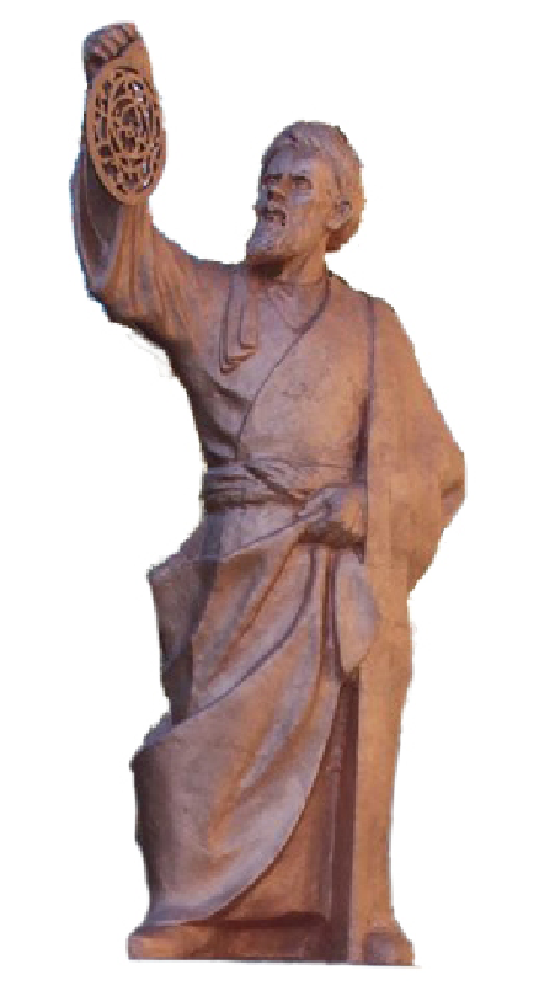
\includegraphics[scale=0.25]{Al-Khwarizmi.eps}\\
\emph{{\small Al-Khwarizmi}}\\
\href{http://fr.wikipedia.org/wiki/Al-Khwarizmi}{http://fr.wikipedia.org/wiki/Al-Khwarizmi}\\[5mm]
\end{center}


3037-- What main subject is covered in `` \emph{Euclid's Elements} '', \ written by Euclid himself?\\

a) arithmetic\\
b) geometry\\
c) optimization\\
d) statistics\\

Answer: b)\\

Explanation:\\
`` \emph{Euclid's Elements} '' \ is a collection of geometric knowledge from Ancient Greece. This was the main study topic for mathematicians of that time period. Thus, the correct answer is b). The collection is divided into 13 volumes.\\
\begin{center}
\begin{tabular}{|c|c|} \hline
{\bf Book numbers} & {\bf Content} \\ \hline \hline
1 to 6 & Geometry Plane \\ \hline
7 to 9 & Relationship Theory \\ \hline
10 & Theory of Irrational Numbers \\ \hline
11 to 13 & Geometry of Space \\ \hline
\multicolumn{2}{c}{}
\end{tabular}
\end{center}
Note that the geometry learned in primary and secondary school is called Euclidian space. There also exists other types of Geometry, for example, hyperbolic and spherical.\\



3038-- Which French mathematician was the first to introduce the symbol ``$\angle$'' to name an angle?\\

a) Adrien-Marie Legendre\\
b) Breauch\`ete Depoulais\\
c) Charlie Brown\\
d) Pierre H\'erigone\\

Answer: d)\\

Explanation :\\
Pierre H\'erigone introduced many symbolic notations in his six volume collection, `` \emph{A compendium of elementary mathematics} ''. He also introduced the symbol for angle measurement, ``$\angle$''. Thus, the correct answer is d). (Furthermore, he introduced the symbol ``$\perp$'' that represents the fact that two straight lines are perpendicular.)\\



3039-- A mathematic problem is said to be \emph{open} when it's solution is unknown.\\
In the 1940's, in a class in the doctorate's program at the University of Berkeley, a professor writes two open statistics problems on the chalkboard. Then, a late-arriving student writes these problems down believing them to be part of a homework assignment. It took him only a couple of days to resolve these problems.  Who was this student?\\

a) Bhaskara I\\
b) Hitmust Biagenius\\
c) Georges Dantzig\\
d) Pythagoras\\

Answer: c)\\

Explanation:\\
It was Georges Dantzig, an American mathematician who solved these problems. As he had arrived late to class, he believed that they were homework problems. The correct answer is c). While doing his homework, he had developed without knowing it, a resolution method able to solve optimization problems.\\

\begin{center}
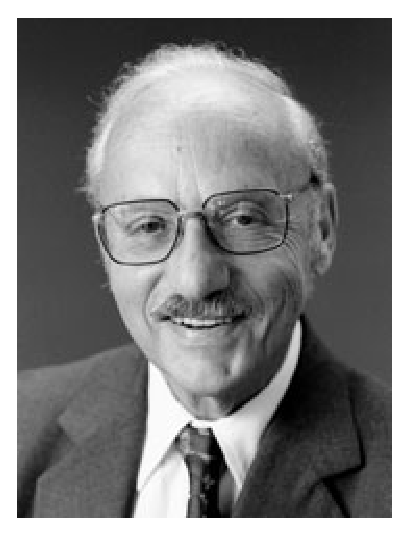
\includegraphics[scale=0.3]{dantzig.eps}\\
\emph{{\small Georges Dantzig}}\\
\href{http://www.siam.org/news/news.php?id=928}{www.siam.org/news/news.php?id=928}\\[5mm]
\end{center}



3040-- According to the legend, in Ancient Greece Thales of Miletos was put to the challenge by Pharaoh Amasis. Name this challenge.\\

a) Calculating the amount of gold coins that could fit in his sarcophagus (type of stone coffin).\\
b) Designing a water reservoir large enough to supply the entire city for one month's time.\\
c) Determining which one was the heaviest construction between the Sphinx and the Great Pyramid of Giza.\\
d) Measuring the height of the Great Pyramid of Giza.\\

Answer: d)\\

Explanation:\\
Pharaoh Amasis would say that no one was able to measure the height of the Great Pyramid of Giza. Thus, the correct answer is d). To obtain the correct calculation, Thales based his argument on the fact that at a certain hour in the day, every object's shadow becomes equal to the height of the same object (Sun rays are thus inclined to 45$^\circ$).  He chose a moment on a specific day and he used his own size to measure the shadow of the Great Pyramid to which he had added half of the length of the pyramid's base. He calculated 85 thales which is equal to 276.25 Egyptian Royal Cubits. In reality, the pyramid is approximately 280 Royal Egyptian Cubits (137 meters) high which is an excellent estimate for that time period.\\
\begin{center}
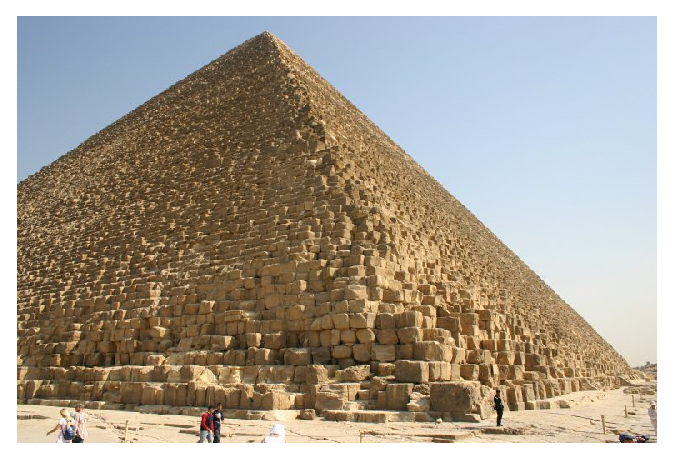
\includegraphics[scale=0.5]{pyramide.eps}\\
\emph{{\small Grande Pyramide de Kh\'eops}}\\
\href{http://fr.wikipedia.org/wiki/Pyramide de Kh\%C3\%A9ops}{fr.wikipedia.org/wiki/Pyramide de Kh\'eops}\\[5mm]
\end{center}



3041-- Up until the 19th century, mathematicians were not called mathematicians. What was their previous name?\\

a) surveyors\\
b) calculators\\
c) geometricians\\
d) measurers\\

Answer: c)\\

Explanation:\\
Up until the 19th century, mathematicians were called geometricians. The correct answer is c). Geometricians like mathematicians focused their studies on volume, area, and length calculations. By definition, a geometrician is also a surveyor, someone who measures land masses.\\



3042-- There exists many types of geometry: Euclidean geometry, hyperbolic, spherical, \dots \ \ What is fundamental to all types of geometry, in other words, what defines geometry?\\

a) the figures we can trace\\
b) angle measurements\\
c) an axiomatic system\\
d) the type of coordinates\\

Answer: c)\\

Explanation:\\
Axioms are general rules that define a type of geometry. They are always precise in the type of geometry that they define, but they can be imprecise in another type. They are used to demonstrate different theorems. The correct answer is c).\\



3043-- Historically, Euclidean geometry was the first type invented. The following diagram:
\begin{center}
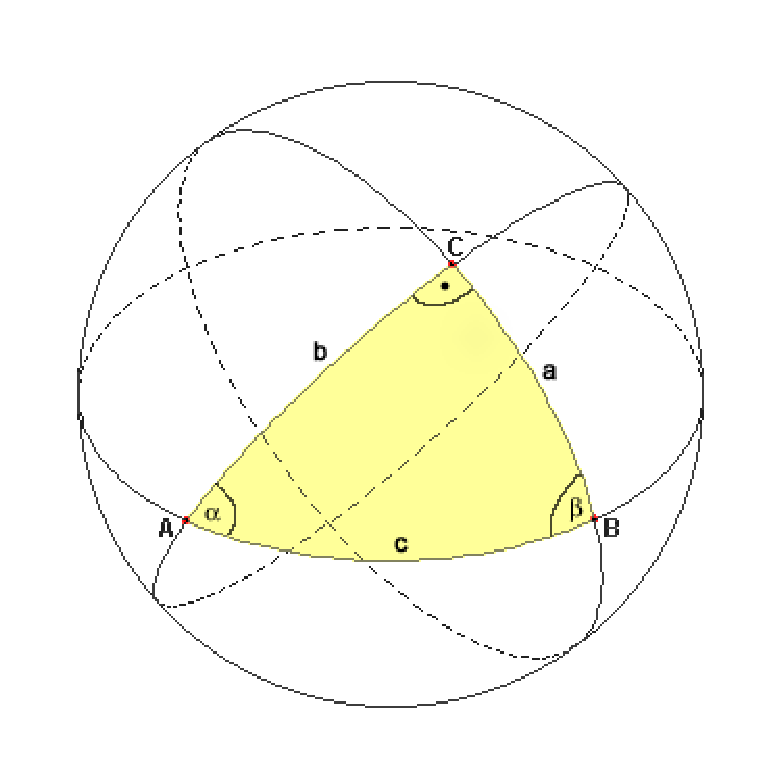
\includegraphics[scale=0.5]{geospher.eps}\\
\href{http://fr.wikipedia.org/wiki/Trigonom\%C3\%A9trie sph\%C3\%A9rique}{fr.wikipedia.org/wiki/}\\[5mm]
\end{center}
and the following axiom: `` There is no straight line that passes through Point $A$ that is also parallel to straight line $a$, in other words, all straight lines passing through Point $A$ cut through straight line $a$ '', describes what type of geometry?\\

a) affine\\
b) hyperbolic\\
c) projective\\
d) spherical\\

Answer: d)\\

Explanation:\\
Like the name indicates, spherical geometry is a set of points and straight lines on a sphere. The correct answer is d). More specifically, a segment of a straight line is the shortest path between two points on a sphere.\\



3044-- Which of the following mathematicians is not considered to be one of the greatest geometricians of Ancient History?\\

a) Apollonius of Perga (262 - 180 B.C.)\\
b) Archimedes of Syracuse (287 - 212 B.C.)\\
c) Aristotle (384 - 322 B.C.)\\
d) Euclid (365 - 275 B.C.)\\

Answer: c)\\

Explanation:\\
Apollonius of Perga is known for his writings on conic sections.\\
\begin{center}
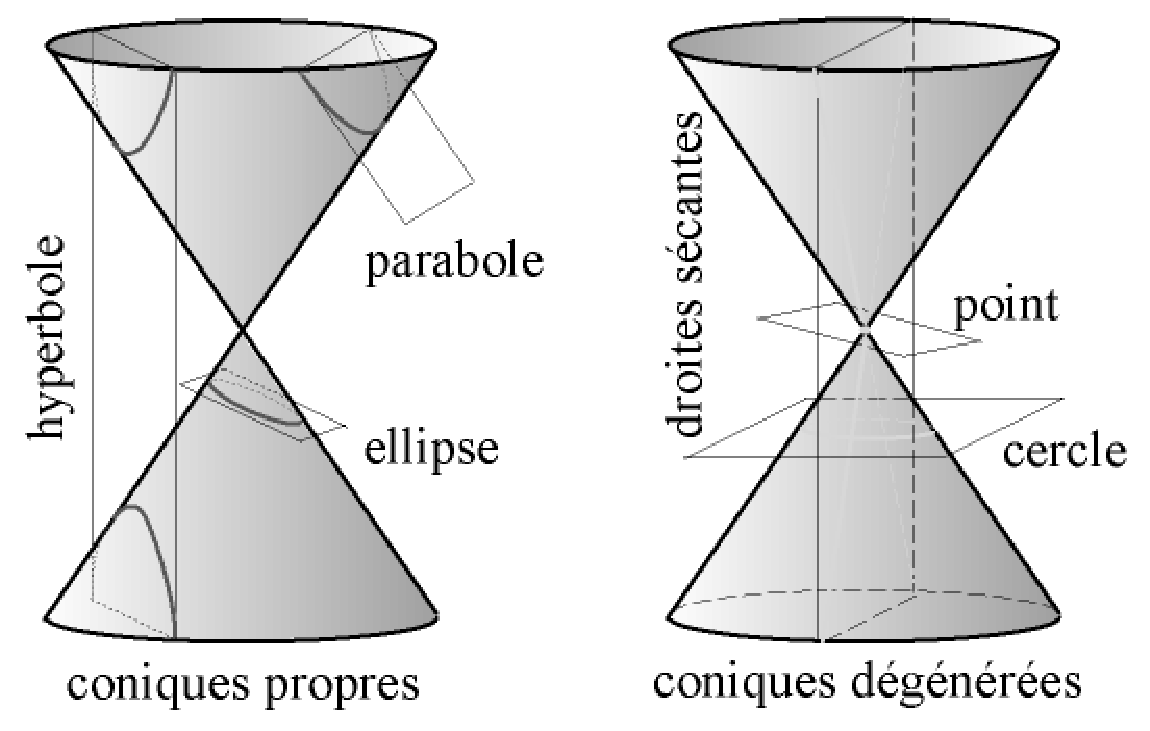
\includegraphics[scale=0.25]{Coniques.eps}\\
\emph{{\small Conique d'Apollonius}}\\
\href{http://fr.wikipedia.org/wiki/Coniques}{fr.wikipedia.org/wiki/Coniques}\\
\end{center}
Archimedes of Syracuse studied conic sections, the calculation of areas, volumes and spirals (the Archimedean spiral).\\
\begin{center}
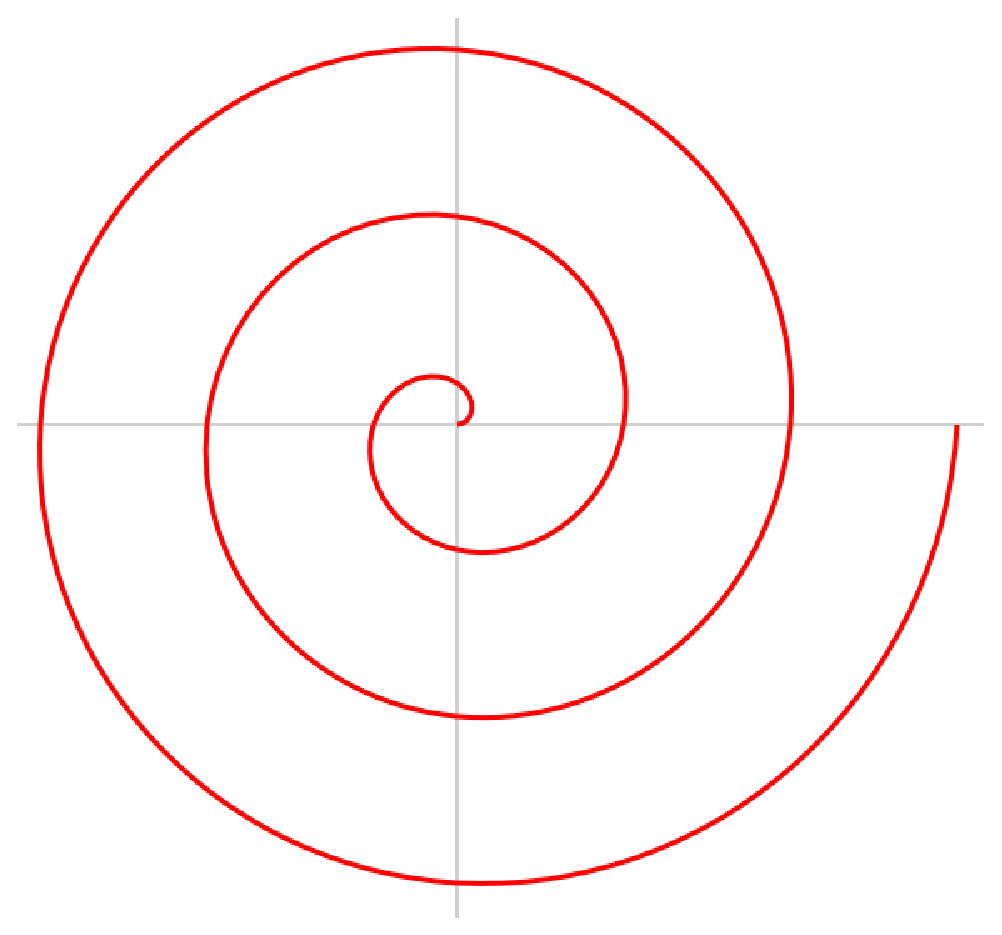
\includegraphics[scale=0.25]{spirale.eps}\\
\emph{{\small Archimedean Spiral}}\\
\href{http://fr.wikipedia.org/wiki/Spirale_d\%27Archim\%C3\%A8de}{fr.wikipedia.org/wiki/Spirale d'Archim\`ede}
\end{center}
%\emph{\textsf{animation qui montrerait la formation de la spirale}}\\
Aristotle, considered to be a great thinker, was not considered to be a great geometrician of his time. He was rather known as a great philosopher. The correct answer is c).\\
Euclid is most well-known for his book `` \emph{Euclid's Elements} '', a collection of geometrical knowledge.\\



3045-- Historically, the main problem that mathematicians had with the number $\pi$ was choosing one symbol to represent it.\\
True or False?\\

Answer: False\\

Explanation:\\
The biggest problem with the number $\pi$ wasn't in choosing the right symbol to represent it but rather in finding it's true value. Many mathematicians have searched and still search to determine the exact decimals of $\pi$. Thus, the correct answer is: False. In September 2002, one could count $1 \, 241 \, 100 \, 000 \, 000$ decimals for $\pi$.\\
\begin{center}
\begin{tabular}{|c|c|c|c|} \hline
{\bf Name} & {\bf Year} & {\bf Exact number of decimals for $\pi$} \\ \hline \hline
Babylonians & -2000 & 1 \\ \hline
Egyptians & -1650 & 1 \\ \hline
Chinese & -1200 & 0 \\ \hline
Archimedes & -250 & 3 \\ \hline
Ptolemy & 150 & 3 \\ \hline
Al-Khwarizmi & 800 & 3 \\ \hline
Fran\c cois Viete & 1593 & 9 \\ \hline
John Machin & 1706 & 100 \\ \hline
Rutherford & 1853 & 440 \\ \hline
Nicholson et Jeenel & 1945 & 3092 \\ \hline
Guilloud et Bouyer & 1973 & $1 \, 001 \, 250$ \\ \hline
Kanada & 2002 & $1 \, 241 \, 100 \, 000 \, 000$\\ \hline
\end{tabular}\\[2mm]
Information taken from the following website: \href{http://www.pi314.net/historique.php}{http://www.pi314.net/historique.php}\\[5mm]
\end{center}
%{\bf \textsf{animation : petit bonhomme \'ebahit, \'etourdit par le nombre de d\'ecimales}}\\



3046-- In 1765, the German mathematician Johann Heinrich Lambert revealed a new property of $\pi$. What was it?\\

a) $\pi = 3,1416$\\
b) $\pi$ is an irrational number\\
c) $\pi$ is a rational number\\
d) $\pi$ has a very large, but finite number of decimals\\

Answer: b)\\

Explanation:\\
Johann Heinrich Lambert proved that $\pi$ is irrational, in other words, there is no exact decimal notation of $\pi$ there only exists approximations. The correct answer is b).\\
\begin{center}
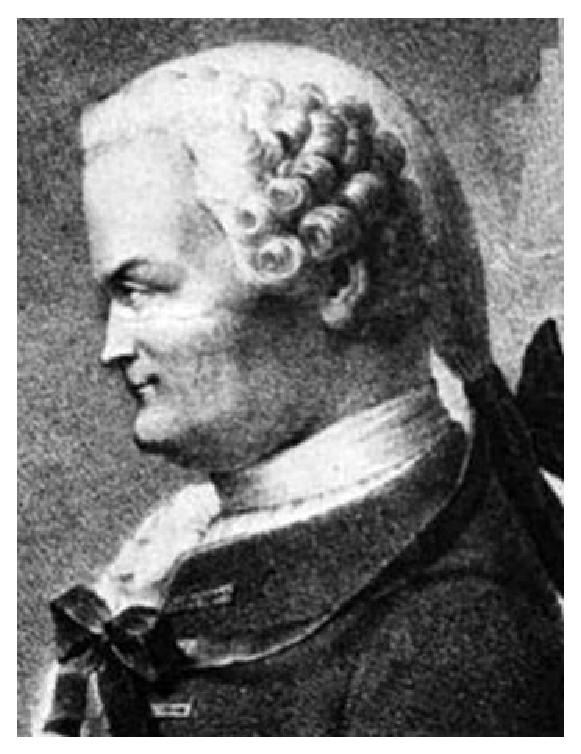
\includegraphics[scale=0.25]{JHLambert.eps}\\
\emph{{\small Johann Heinrich Lambert}}\\
\href{http://fr.wikipedia.org/wiki/Johann Heinrich Lambert}{fr.wikipedia.org/wiki/Johann Heinrich Lambert}\\[5mm]
\end{center}



3047-- Which English mathematician was the first to use the greek letter $\pi$ to name this amount: 3.141 592 654 \dots ?\\

a) Apollonius of Perga\\
b) Scipione del Ferro\\
c) Sun Zi\\
d) William Jones\\

Answer: d)\\

Explanation:\\
In 1706, William Jones proposed in his literary work `` \emph{A New Introduction to Mathematics} '' \ the usage of the $\pi$ symbol to represent the relationship between the circonference of a circle and its diameter:
\begin{eqnarray*}
\pi &=& \frac{\textrm{circonf\'erence}}{\textrm{diam\`etre}}\\[2mm]
 &=& \frac{2\pi r}{d}\\[2mm]
 &=& \frac{d\pi}{d}
\end{eqnarray*}
Thus, the correct answer is d). Leonhard Euler used one of these symbols in 1748 in one of his works.

\begin{center}
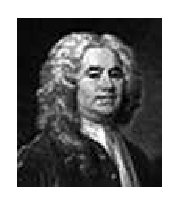
\includegraphics[scale=1]{William_Jones.eps}\\
\emph{{\small William Jones}}\\
\href{http://fr.wikipedia.org/wiki/William Jones \%28math\%C3\%A9maticien\%29}{fr.wikipedia.org/wiki/William Jones (mathematicien)}\\[5mm]
\end{center}



3048-- Between which two centuries did the mathematical operation ``exponentiation''  $x^{m+n} = x^{m} \cdot x^{n}$ appear?\\

a) 5th and 6th centuries\\
b) 11th and 12th centuries\\
c) 14th and 15th centuries\\
d) 21st and 22nd centuries\\

Answer: b)\\

Explanation:\\
Arabs invented exponentiation rules between 1000 and 1200 A.D. Thus, the correct answer is b). Arabs invented these rules between the 11th and 12th centuries. In that time period, Arabs wrote their algebraic equations in words and not in symbols.\\



3049-- Who invented the algorithm for polynomial division?\\
For example,
\begin{center}
\begin{tabular}{r}
$x^{2} - 1$ \ \ \ \ \ \ \\
\underline{$- (x^{2} + x)$} \ \ \ \  \ \\
$- x - 1$ \ \\
\underline{$- (-x - 1)$}\\
$0$ \
\end{tabular}
\begin{tabular}{|c}
$x + 1$ \\ \hline
$x - 1$\\
\\
\\
\\
\end{tabular}
\end{center}
%\textsf{animation : bonhomme pourrait effectuer la division??}\\

a) Arabs\\
b) Chinese\\
c) French from the Renaissance period\\
d) Italians from the Renaissance period\\

Answer: a)\\

Explanation:\\
Between 1000-1200 A.D., Arabs invented the polynomial division algorithm. The correct answer is a). Their method can even handle negative powers in polynomials.\\
\begin{center}
\begin{tabular}{r}
$x^{2} + 1$ \ \ \ \ \ \ \ \ \ \ \ \ \ \ \ \ \ \ \ \ \ \ \ \\
\underline{$- (x^{2} + 2x)$} \ \ \ \ \ \ \ \ \ \ \ \ \ \ \ \ \ \ \ \ \\
$- 2x + 1$ \ \ \ \ \ \ \ \ \ \ \ \ \ \ \ \\
\underline{$- (-2x - 4)$} \ \ \ \ \ \ \ \ \ \ \ \ \ \ \\
$5$ \ \ \ \ \ \ \ \ \ \ \ \ \ \ \ \\
\underline{$- (5 + 10/x)$} \ \ \ \ \\
$-10/x$ \ \ \ \ \ \\
$\vdots$ \ \ \ \ \ \ \ \ \ \
\end{tabular}
\begin{tabular}{|c}
$x + 2$ \\ \hline
$x - 2 + 5/x - 10/x^{2} \cdots$\\
\\
\\
\\
\\
\\
\\

\end{tabular}\\
\end{center}



3050-- Al-Khwarizmi is considered arguably to be the Father of Algebra. In his book, `` \emph{al-jabr wa'l muqabala} '' he uses the word `` \emph{shai} '', thing, to represent a variable. Which of the following words was never used to designate a variable?\\

a) causa\\
b) cosa\\
c) cose\\
d) coss\\

Answer: c)\\

Explanation:\\
A few Latin texts use the word `` \emph{causa} '' for Al-Khwarizmi's word `` \emph{shai} ''. Translated into Italian, `` \emph{causa} '' becomes `` \emph{cosa} '' and into German `` \emph{coss} ''. `` \emph{Cose} '' was never used to designate a variable. The correct answer is c).\\



3051--
\begin{center}
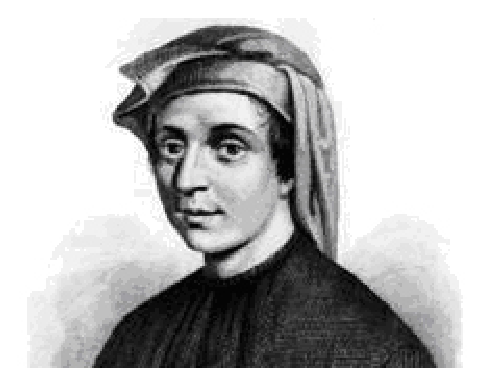
\includegraphics[scale=0.4]{Fibonacci.eps}\\
\emph{{\small L\'eonardo of Pisa {\scriptsize dit} Fibonacci}}\\
\href{http://fr.wikipedia.org/wiki/Fibonacci}{fr.wikipedia.org/wiki/Fibonacci}\\
\end{center}

During the time period of Leonardo of Pisa (1170-1250), an algebraic equation was still written in words. For example:\\
\begin{quote}
`` \emph{A cube and eight things minus five squares is equal to the root of one plus one thing.}''\\
\end{quote}
How would this equation be written today?\\

a) $x^{3} - 5x^{2} + 8 = \sqrt{x} + 1$\\[2mm]
b) $x^{3} - 5x^{2} + 8 = \sqrt{x + 1}$\\[2mm]
c) $x^{3} - 5x^{2} + 8x = \sqrt{x} + 1$\\[2mm]
d) $x^{3} - 5x^{2} + 8x = \sqrt{x + 1}$\\

Answer: d)\\

%\emph{\textsf{animation : petit bonhomme d\'eguis\'e en magicien, prend chaque expression en mots et la transforme en symbole}}\\
Explanation:\\
\begin{center}
\begin{tabular}{|c|c|}\hline
A cube & $x^{3}$\\ \hline
and & $+$\\ \hline
eight things & $8x$\\ \hline
minus five squares & $-5x^{2}$\\ \hline
is equal to & $=$\\ \hline
the root of one plus one thing & $\sqrt{x + 1}$\\ \hline
\end{tabular}\\[4mm]
$\Longrightarrow \ \ \ \ \ \ \ x^{3} + 8x - 5x^{2} = \sqrt{x + 1} \ \ \ \ \ \ \ \Longleftrightarrow \ \ \ \ \ \ \ x^{3} - 5x^{2} + 8x = \sqrt{x + 1}$
\end{center}
Thus, the correct answer is d).\\


3052-- Which of the following is the proper name used to designate the study of algebraic equations?

a) `` \emph{Art of The Thing} ''\\
b) `` \emph{Cossic Art} ''\\
c) `` \emph{Equations Art} ''\\
d) `` \emph{The Thing and its Art} ''\\

Answer: b)\\

Explanation:\\
Algebraic equation writing was done in words and not in symbols; it was very complex and considered to be an art. The English were inspired by the word `` \emph{coss} '', thing, that for German mathematicians implied the designation of a variable. Thus, `` \emph{coss} '', `` \emph{cossic} '', hence its name: `` \emph{Cossic Art} ''. The correct answer is b).\\



3053-- In what year did `` \emph{Summa Aritmetica} '', a book written by the Italian monk Luca Pacioli, get published?\\

a) 1494\\
b) 1724\\
c) 1894\\
d) 2006\\

\begin{center}
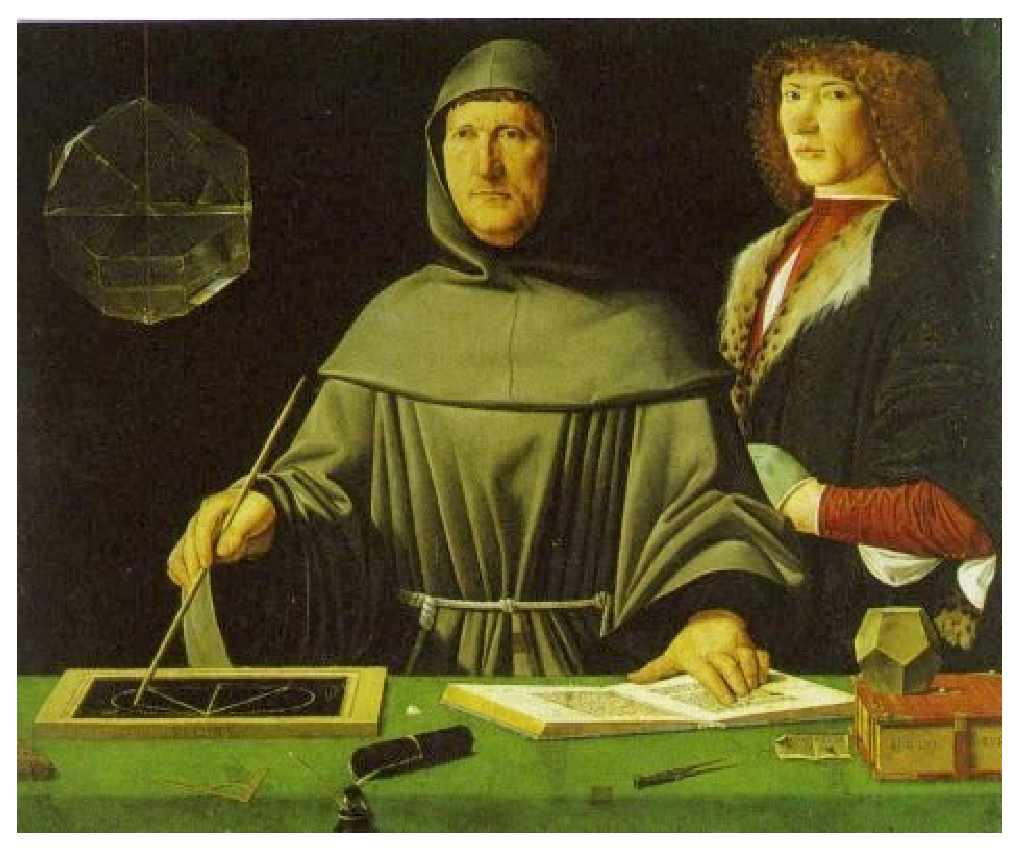
\includegraphics[scale=0.25]{Pacioli.eps}\\
\emph{{\small Luca Pacioli}}\\
\href{http://fr.wikipedia.org/wiki/Luca Pacioli}{fr.wikipedia.org/wiki/Luca Pacioli}\\
\end{center}

Answer: a)\\

Explanation:\\
`` \emph{Summa Aritmetica} '' was published in 1494. The answer is a). This book would serve as a main introductive source to the symbolic art of algebraic equations.\\



3054-- The main problem with Luca Pacioli's notation is that in an algebraic equation, one can only express one unknown at once. This type of equation would look something like this:\\
\begin{eqnarray*}
cu.\tilde{m}.5.ce.\tilde{p}.7.co.\textrm{------}\mathcal{R}v.co.\tilde{p}.6.
\end{eqnarray*}
True or False?\\

Answer: True\\

Explanation:\\
\begin{eqnarray*}
cu.\tilde{m}.5.ce.\tilde{p}.7.co.\textrm{------}\mathcal{R}v.co.\tilde{p}.6.
\end{eqnarray*}
The abbreviation `` $co$ '' \ represents `` \emph{cosa} '', thing, or the unknown quantity. `` $ce$ '' and `` $cu$ '' are respectively `` \emph{censo} ''  and `` \emph{cubo} '', from the Italian square and cube. `` $v$ '' means `` \emph{universal} ''. It regroups all of the terms that follow it. For example, `` \emph{co} '' refers to a single unknown quantity. The weakness of this notation is in the impossibility of representing more than one unknown at a time. The correct answer is: True. In current notation, the expression would be written:\\
\begin{eqnarray*}
cu.\tilde{m}.4.ce.\tilde{p}.10.co.\textrm{------}\mathcal{R}v.co.\tilde{p}.3. \ \ \Longleftrightarrow \ \ x^{3} - 4x^{2} + 10x = \sqrt{x + 3}
\end{eqnarray*}\\



3055-- In 1484, which French mathematician created his own notation for algebraic expressions and exponents?\\

a) Beno\^it Mandelbrot\\
b) Bob Barker\\
c) Joseph Liouville\\
d) Nicolas Chuquet\\

Answer: d)\\

Explanation:\\
Nicolas Chuquet wrote `` \emph{Triparty en la science des nombres} '', a book about algebra in which he created different notations in order to clarify the art of working with algebraic expressions. He invented such terms as:\\
\begin{eqnarray*}
5^{2} \ \ \ \ \ \text{which is now written:} \ \ \ \ \ 5x^{2}.\\
\mathcal{R}^{3} 5 \ \ \ \ \ \text{which is now written:} \ \ \ \ \ \sqrt[3]{5}.
\end{eqnarray*}
The correct answer is d).\\



3056-- Nicolas Chuquet never published `` \emph{Triparty en la science des nombres} '' in his lifetime. One of his students published `` \emph{L'arismetique} '' which in fact is a copy of Chuquet's book. Who is this copying French mathematician?\\

a) Atomic Betty\\
b) Estienne de La Roche\\
c) Pythagoras\\
d) Ren\'e Descartes\\

Answer: b)\\

%\emph{\textsf{animation : p'tit bonhommme pourrait passer, d\'eguis\'e en voleur, avec un livre sous le bras...}}\\
Explanation:\\
It was Estienne de La Roche who published `` \emph{L'arismetique} '', a copy of `` \emph{Triparty en la science des nombres} '', in 1520. The correct answer is b). Only in 1880 was Chuquet's work officially published for the first time.\\



3057-- To which French mathematician do we owe the following large number system?\\
\begin{center}
\begin{tabular}{|c|c|c|c|} \hline
{\bf Base of 10} & {\bf Power} & {\bf Name given by \dots} & {\bf Notation by \dots} \\ \hline \hline
$10^{0}$ & million$^{0}$ & unit & 1\\[1mm] \hline
$10^{3}$ & million$^{0.5}$ & thousand & 1000\\[1mm] \hline
$10^{6}$ & million$^{1}$ & million & 100000\\[1mm] \hline
$10^{9}$ & million$^{1.5}$ & thousand million & 100.000000\\[1mm] \hline
$10^{12}$ & million$^{2}$ & billion & 100000.000000\\[1mm] \hline
$10^{15}$ & million$^{2.5}$ & thousand billion & 100.000000.000000\\[1mm] \hline
$10^{18}$ & million$^{3}$ & trillion & 100000.000000.000000\\[1mm] \hline
\multicolumn{4}{c}{}\\
\end{tabular}\\
\end{center}
This first notation uses points to separate a large number into sets of six digits. Today, in English notation, dots are still used to separate large numbers but in sets of three digits, not six. In French notation, however, spaces are used to separate large numbers in sets of three digits.\\

a) Blaise Pascal\\
b) Joseph Liouville\\
c) Nicolas Chuquet\\
d) Pafnouti Tchebychev\\

Answer: c)\\

Explanation:\\
Nicolas Chuquet had the idea of regrouping large numbers in sets of six and separating them with dots. The correct answer is c). At the beginning of the 17th century, large numbers were divided into groups of three instead of six to enhance readability. Still today, in the English number system, dots are used to separate numbers in groups of three (however, in the French number system, spaces are now used instead of dots). Today, the names given by Chuquet are known as the "long scale" in the English language. \\
\begin{center}
\begin{tabular}{|c|c|c|c|} \hline
{\bf Base of 10} & {\bf Power} & {\bf Name given by Chuquet} & {\bf Chuquet's notation} \\ \hline \hline
$10^{0}$ & million$^{0}$ & unit & 1\\[1mm] \hline
$10^{3}$ & million$^{0.5}$ & thousand & 1000\\[1mm] \hline
$10^{6}$ & million$^{1}$ & million & 100000\\[1mm] \hline
$10^{9}$ & million$^{1.5}$ & thousand million & 100.000000\\[1mm] \hline
$10^{12}$ & million$^{2}$ & billion & 100000.000000\\[1mm] \hline
$10^{15}$ & million$^{2.5}$ & thousand billion & 100.000000.000000\\[1mm] \hline
$10^{18}$ & million$^{3}$ & trillion & 100000.000000.000000\\[1mm] \hline
\multicolumn{4}{c}{}\\
\end{tabular}\\
\end{center}



3058-- Which French mathematician invented new names for the groups of three-digit large numbers?\\
\begin{center}
\begin{tabular}{|c|c|c|} \hline
{\bf Base of 10} & {\bf Power} & {\bf Name given by Peletier du Mans} \\ \hline \hline
$10^{0}$ & million$^{0}$ & unit \\[1mm] \hline
$10^{3}$ & million$^{0.5}$ & thousand \\[1mm] \hline
$10^{6}$ & million$^{1}$ & million \\[1mm] \hline
$10^{\bf{9}}$ & million$^{\bf{1.5}}$ & \textbf{milliard} \\[1mm] \hline
$10^{12}$ & million$^{2}$ & billion \\[1mm] \hline
$10^{\bf{15}}$ & million$^{\bf{2.5}}$ & \textbf{billiard} \\[1mm] \hline
$10^{18}$ & million$^{3}$ & trillion \\[1mm] \hline
$10^{\bf{21}}$ & million$^{\bf{3.5}}$ & \textbf{trilliard} \\[1mm] \hline
\multicolumn{3}{c}{}\\
\end{tabular}\\
\end{center}

a) Isaac Newton\\
b) Jacques Peletier du Mans\\
c) Nicolas Chuquet\\
d) William Brouncker\\

Answer: b)\\

Explanation:\\
Jacques Peletier du Mans proposed different new names for the large intermediate numbers (of three digits). Note that the world "milliard" exists in may languages, but is unknown to American English and not used in British English. The correct answer is b).
\begin{center}
\begin{tabular}{|c|c|c|} \hline
{\bf Base of 10} & {\bf Power} & {\bf Name given by Peletier du Mans} \\ \hline \hline
$10^{0}$ & million$^{0}$ & unit \\[1mm] \hline
$10^{3}$ & million$^{0.5}$ & thousand \\[1mm] \hline
$10^{6}$ & million$^{1}$ & million \\[1mm] \hline
$10^{\bf{9}}$ & million$^{\bf{1.5}}$ & \textbf{milliard} \\[1mm] \hline
$10^{12}$ & million$^{2}$ & billion \\[1mm] \hline
$10^{\bf{15}}$ & million$^{\bf{2.5}}$ & \textbf{billiard} \\[1mm] \hline
$10^{18}$ & million$^{3}$ & trillion \\[1mm] \hline
$10^{\bf{21}}$ & million$^{\bf{3.5}}$ & \textbf{trilliard} \\[1mm] \hline
\multicolumn{3}{c}{}\\
\end{tabular}\\
\end{center}



3059-- In the 1600's, many mathematicians invented symbolic notations for algebraic expressions. Associate each mathematician with the notation that he invented.\\
\begin{center}
\begin{tabular}{|c|c|} \cline{2-2}
\multicolumn{1}{c|}{} & \multicolumn{1}{|c|}{\bf Notation}\\ \hline
1) & $4aaa + 7ee$\\ \hline
2) & $4a3 + 7e2$\\ \hline
3) & $4a^{iii} + 7e^{ii}$\\ \hline
4) & $4a^{3} + 7e^{2}$\\ \hline
\end{tabular} \ \ \ \ \ \ \ \
\begin{tabular}{|c|l|} \cline{2-2}
\multicolumn{1}{c|}{} & \multicolumn{1}{|c|}{\bf Mathematician}\\ \hline
A) & 1620 - Thomas Harriot\\ \hline
B) & 1634 - Pierre H\'erigone\\ \hline
C) & 1636 - James Hume\\ \hline
D) & 1637 - Ren\'e Descartes\\ \hline
\end{tabular}
\end{center}

a) 1-A; 2-B; 3-C; 4-D\\
b) 1-B; 2-C; 3-A; 4-D\\
c) 1-C; 2-A; 3-D; 4-B\\
d) 1-D; 2-C; 3-A; 4-D\\

Answer: a)\\

%{\bf \textsf{animation: petit bonhomme pourrait \^etre comme la miss Roue de Fortune et d\'evoiler les bonnes r\'eponses}}\\
Explanation:\\
\begin{center}
\begin{tabular}{|c|c|l|} \cline{2-3}
\multicolumn{1}{c|}{} & \multicolumn{1}{|c|}{\bf Notation} & \multicolumn{1}{|c|}{\bf Mathematician}\\ \hline
1-A & $4aaa + 7ee$ & 1620 - Thomas Harriot\\ \hline
2-B & $4a3 + 7e2$ & 1634 - Pierre H\'erigone\\ \hline
3-C & $4a^{iii} + 7e^{ii}$ & 1636 - James Hume\\ \hline
4-D & $4a^{3} + 7e^{2}$ & 1637 - Ren\'e Descartes\\ \hlinex
\end{tabular}\\
\end{center}
The correct answer is a).\\



3060-- Which 17th century French mathematician introduced the usage of first letters of the alphabet for constants $(a,\,b,\,c,\,\dots)$ and last letters of the alphabet for variables ($x,\,y,\,z$)?\\

a) Bartholomew J. Simpson\\
b) Galileo Galilei\\
c) Pierre Fatou\\
d) Ren\'e Descartes\\

Answer: d)\\

Explanation:\\
In addition to inventing the following notation: $5x^{3} - 8y^{2}$, otherwise known as exponents used to express powers, Ren\'e Descartes invented the usage of letters from the alphabet: constants, by the first letters of the alphabet ($a, b, c, \dots$)  and variables, by the last letters of the alphabet  ($x, y, z$). The correct answer is d).\\
\begin{center}
\includegraphics[scale=0.4]{Descartes.eps}\\
\emph{{\small Ren\'e Descartes}}\\
\href{http://fr.wikipedia.org/wiki/Ren\%C3\%A9 Descartes}{fr.wikipedia.org/wiki/Ren\'e Descartes}\\[5mm]
\end{center}

3061-- Which 16th century British mathematician invented the equal sign ($=$) as we know it today?\\

a) Bonaventura Cavalieri\\
b) Danny Ocean\\
c) Robert Recorde\\
d) Sofia Kovalevska\"ia\\

Answer: c)\\

Explanation:\\
In 1557, Robert Recorde proposed the usage of  ``$=$'' to designate equality. The correct answer is c). This symbol was used widely throughout England but wasn't very popular in continental Europe. Most likely it was Isaac Newton and Gottfried Wilhelm von Leibniz that contributed the most to the adoption of the symbol ``$=$''.\\

\begin{center}
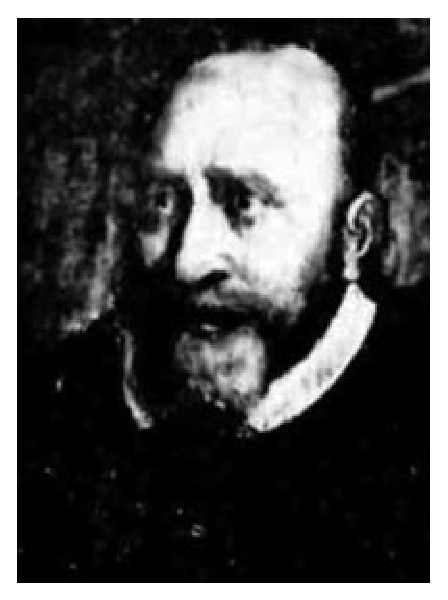
\includegraphics[scale=0.4]{recorde.eps}\\
\emph{{\small Robert Recorde}}\\
\href{http://www.pbs.org/wgbh/nova/einstein/ance-equals.html}{www.pbs.org/wgbh/nova/einstein/ance-equals.html}\\[5mm]
\end{center}



3062-- Which symbol was never used to represent equality ($=$)?\\

a) \includegraphics[scale=0.09]{egaliteDescartes.eps}\\
b) $\sim$\\
c) ------\\
d) $\asymp$\\

Answer: d)\\

Explanation:\\
Ren\'e Descartes has invented the symbol \includegraphics[scale=0.09]{egaliteDescartes.eps} to represent equality. Pacioli used the symbol ------. In 18th century literature, one can sometimes come across the symbol $\sim$ (nowadays, $\sim$ designates an approximation). But $\asymp$ was never used to designate equality. The correct answer is d).\\



3063-- Even in Ancient Egypt, scribes already knew how to solve first degree equations. For example:
\begin{center}
`` \emph{A third of a quantity plus itself equals 16.} ''\\
\end{center}
In actual notation, it would be written as: $x + \frac{x}{3} = 16$.\\[2mm]
Scribes proceeded in the following manner:\\
\begin{itemize}
\item They chose a quantity; in this instance it would be 3, for a third of 3 is easy to calculate! \ ($3\times \frac{1}{3} = 1$)
\item 3 plus a third of 3 equals $3 + \frac{3}{3} = 3 + 1 = 4$.
\item 16 is the targeted number but we only are up to 4. So, 4 must be multiplied by 4. ($4 \times 4 = 16$).
\item Since $x = 3$, then $4 \times 3 = 12$.\\
The answer is 12.
\end{itemize}
Let's double check: if $x = 12$, then $x + \frac{x}{3} = 12 + \frac{12}{3} = 12 + 4 = 16$.\\
\\
What is the name of this method?\\

a) Complementary division method\\
b) False position method\\
c) Complete multiplication method\\
d) Substitution method\\

Answer: b)\\

Explanation:\\
This method is called the ``False position method''. It was given this name because the $x$ in the equation does not represent the correct answer, but instead, it is chosen mainly because it is easy to work with. The correct answer is b). Let's bring the equation back to $Ax = B$. It would seem easy to solve this equation, but one must remember that in that time period, fractional calculations and symbolism weren't exactly mastered arts and negative numbers weren't even invented yet.\\



3064-- The double false position method allows us to calculate a first degree equation through the following formula: $Ax + C = B$. Which ethnic group invented this method?\\

a) The Arabs\\
b) The Babylonians\\
c) The Chinese\\
d) The Egyptians\\

Answer: c)\\

Explanation:\\
The Chinese developed the double false position method in order to solve first degree equations through the following formula: $Ax + C = B$. The correct answer is c). Note that the Indians also used this method.\\



3065-- In order to solve a quadratic equations ($ax^{2} + bx + c = 0$), mathematician Al-Khwarizmi used the following formula:
\begin{eqnarray*}
x = \sqrt{\Big(\frac{b}{2}\Big)^{2} + c} \ - \frac{b}{2}
\end{eqnarray*}
In fact, Al-Khwarizmi studied the form of the equation  $x^{2} + bx = c$, in which the constants $b$ and $c$ are positive. Note that this notation did not exist at that time period and that the notation, instead, would have been written in words.\\

The biggest difference between this formula and the one known today
\begin{eqnarray*}
x = \frac{-b \pm \sqrt{b^{2} - 4ac}}{2a}
\end{eqnarray*}
is only in the way it is written.\\
True or False?\\

Answer: False\\

Explanation:\\
In that era, people only accepted positive roots and rejected all negative roots because they did not know about negative numbers yet. Nowadays, these two types of roots are both accepted, hence the arrival of the  $\pm$ sign. Thus, the biggest difference between these two formulas isn't in the way that they are written but rather in the fact that they are both considered as two distinct roots. The correct answer is: False.\\



%trop longue
%3066-- Soit l'\'equation quadratique suivante:
%\begin{eqnarray}
%x^{2} + 8x = 20
%\end{eqnarray}
%Quelles sont les racines enti\`eres positives de cette \'equation?\\
%Un math\'ematicien a r\'esolu ce probl\`eme de la fa\c con g\'eom\'etrique. Voici comment il a proc\'ed\'e:


%\begin{enumerate}
%\item On dessine un carr\'e de c\^ot\'e $x$, donc d'aire $x^{2}$, auquel on colle un rectangle d'aire $8x$. On a maintenant un rectangle d'aire $x^{2} + 8x = 20$ (de l'\'equation (1)).
%\begin{center}
%\includegraphics[scale=0.15]{rectx28x.eps}\\
%figure 1\\
%\end{center}

%\item On divise en deux le rectangle d'aire $8x$, sur la hauteur et on forme la figure 3 :
%\begin{center}
%\begin{tabular}{c c}
%\includegraphics[scale=0.15]{rect8x.eps} \ \ \ \ \  & \ \ \ \ \ \includegraphics[scale=0.15]{carreincomp.eps}\\
%figure 2 & figure 3\\
%\end{tabular}
%\end{center}
%L'aire de la figure 3 est toujours de 20.

%\item On compl\`ete la figure 3 par un petit carr\'e d'aire 16 ($4\times 4$).
%\begin{center}
%\includegraphics[scale=0.15]{carrecomp.eps}\\
%figure 4\\
%\end{center}

%\item Une fois le carr\'e complet\'e, on obtient son aire en additionnant l'aire de la figure 3 et l'aire du petit carr\'e $4\times 4$ :
%\begin{center}
%aire de la figure 4 = aire de la figure 3 + aire du petit carr\'e = $20 + 16 = 36$.
%\end{center}
%La figure 4 est un carr\'e de c\^ot\'e de longueur 6 ($\sqrt{36} = 6$).
%\begin{center}
%\includegraphics[scale=0.15]{carrcarre.eps}\\
%figure 5\\
%\end{center}

%\item Donc on peut trouver la valeur de $x$ :
%\begin{eqnarray*}
%x + 4 = 6 \ \ \Rightarrow \ \ x = 6 - 4 = 2.
%\end{eqnarray*}
%\end{enumerate}

%Quel math\'ematicien a invent\'e cette m\'ethode et s'en est servi pour d\'emontrer les solutions des \'equations quadratiques\\

%a) Al-Khwarizmi\\
%b) Blaise Pascal\\
%c) Archim\`ede de Syracuse\\
%d) Carl Friedrich Gauss\\

%R\'eponse : a)\\

%R\'etroaction :\\
%Al-Khwarizmi a utilis\'e cette m\'ethode pour montrer qu'une \'equation quadratique de la forme\\
%$x^{2} + bx = c$ a une solution de la forme $\sqrt{\Big(\frac{b}{2}\Big)^{2} + c} \ - \frac{b}{2}$. La r\'eponse est a).
%\begin{center}
%\includegraphics[scale=0.2]{Al-Khwarizmi.eps}\\
%\emph{{\small Al-Khwarizmi}}\\
%\href{http://fr.wikipedia.org/wiki/Al-Khwarizmi}{fr.wikipedia.org/wiki/Al-Khwarizmi}\\
%\end{center}



3066-- Around 500 B.C., geometry was at the heart of mathematics. Numbers were often associated with figures:
\begin{center}
\begin{tabular}{|c|c|c|c|c|} \hline
{\bf Type of number} & \multicolumn{4}{c|}{\bf Examples}\\[2mm] \hline
triangular numbers& & & & \\
& \includegraphics[scale=0.2]{nbtriangle1.eps} & \includegraphics[scale=0.2]{nbtriangle3.eps} & \includegraphics[scale=0.2]{nbtriangle6.eps} & \dots\\[2mm] \hline
square numbers & & & \\
& \includegraphics[scale=0.2]{nbcarre1.eps} & \includegraphics[scale=0.2]{nbcarre4.eps} & \includegraphics[scale=0.2]{nbcarre9.eps} & \dots\\[2mm] \hline
pentagonal numbers & & & & \\
& \includegraphics[scale=0.2]{nbpenta1.eps} & \includegraphics[scale=0.2]{nbpenta5.eps} & \includegraphics[scale=0.2]{nbpenta12.eps} & \dots\\[2mm] \hline
\end{tabular}\\
\end{center}
For which Greek group was the association of numbers with figures widely accepted?\\

a) The Cyclopses\\
b) The Motards\\
c) The Pythagoreans\\
d) The Tofus\\

Answer: c)\\

Explanation:\\
Pythagoras founded the Pythagorean School around 500 B.C. The students were called Pythagoreans and they philosophized about mathematics. Since geometry was ever-present back then, it was natural for Pythagoreans to associate numbers to geometric figures. The correct answer is c).\\



3067-- Which mathematicians proposed the following solution:
\begin{eqnarray*}
x = \frac{-b \pm \sqrt{b^{2} - 4ac}}{2a}
\end{eqnarray*}
to the quadratic equation $ax^{2} + bx + c = 0$?\\

a) Archimedes of Syracuse and Pythagoras\\
b) Asterix and Obelix\\
c) Andre\"i Markov and Pafnouti Tchebychev\\
d) Thomas Harriot and Ren\'e Descartes\\

Answer: d)\\

Explanation:\\
Thomas Harriot and Ren\'e Descartes realized that it would be easier to write equations as ``things'' equal to zero. The main advantage to this is that the equations $ax^{2} + bx = c$ and $ax^{2} + c = bx$ can be seen as exceptions to the general equation $ax^{2} + bx + c = 0$. So, Harriot and Descartes presented the general solution as follows:
\begin{eqnarray*}
x = \frac{-b \pm \sqrt{b^{2} - 4ac}}{2a}
\end{eqnarray*}
The correct answer is d).
\begin{center}
\begin{tabular}{c c}
\includegraphics[scale=0.25]{harriot.eps} & \includegraphics[scale=0.37]{Descartes.eps}\\
\emph{{\small Thomas Harriot}} & \emph{{\small Ren\'e Descartes}}\\
\href{http://www.luminarium.org/renlit/hariot.htm}{www.luminarium.org/renlit/hariot.htm} & \href{http://fr.wikipedia.org/wiki/Ren\%C3\%A9_Descartes}{fr.wikipedia.org/wiki/Ren\'e Descartes}\\
 & \\
\end{tabular}
\end{center}



3068-- In what time period was the first solution to a cubic (third degree equation) equation problem written?\\

a) Ancient Egypt\\
b) Ancient Greece\\
c) The Middle Ages\\
d) The Renaissance period\\

Answer: b)\\

Explanation:\\
One must go back all the way to 400 B.C. to find the first solution to a cubic equation problem; this geometric problem is of Greek origins. The correct answer is b).\\



3069-- Which problem is at the origin of cubic (to the third degree) equation solutions research?\\

a) the volume calculation problem\\
b) the cube duplication problem (doubling a cube's volume)\\
c) the human sharing problem \\
d) the angle trisection problem (divide one angle into three equal angles)\\

Answer: d)\\

Explanation:\\
The cubic equation solving process began with the angle trisection problem. The correct answer is d). The problem is read as follows:\\
\begin{quote}
\emph{With any given angle $\angle ABC$, there is a way to divide an angle into three equal angles with the help of an unmarked ruler and a compass.}\\
\end{quote}
The answer is \underline{No}; it is impossible to trisect an angle with only an unmarked ruler and a compass.\\
Note that in certain cases trisection would be possible, if the ruler were marked.\\



3070-- According to Omar Khayyam (1048-1131), how many different forms of cubic equations are there if the coefficient of $x^{3}$ is 1, the equation is not null, and the coefficients are positive? (For example, $x^{3} + bx = c, x^{3} = ax^{2} + c$ are a few forms of third degree equations.)
\begin{center}
\includegraphics[scale=0.3]{Omar_Khayyam.eps}\\
\emph{{\small Omar Khayyam}}\\
\href{http://www.nndb.com/people/043/000031947/}{www.nndb.com/people/043/000031947/}\\
\end{center}

a) 6\\
b) 10\\
c) 14\\
d) 19\\

Answer: c)\\

Explanation:\\
In third degree equations, Arabs didn't consider negative numbers to be numbers and they accepted zero as a coefficient, but without allowing an equation to ever be equal to zero. Thus, $x^{3} + bx = c$ and $x^{3} = bx + c$ are two different equations. There are 14 in all. The correct answer is c).
\begin{center}
\begin{tabular}{|l|l|l|l|l|}\hline
$x^{3} = ax^{2} + bx + c$ \ \ \ & $x^{3} + bx + c = ax^{2}$ \ \ \ & $x^{3} + c = ax^{2} + bx$ \ \ \ & $x^{3} + c = bx$ \ \ \ & $x^{3} + c = ax^{2}$ \ \ \ \\ \hline
$x^{3} + ax^{2} + bx = c$ \ \ \ & $x^{3} + ax^{2} = bx + c$ \ \ \ & $x^{3} = bx + c$ \ \ \ & $x^{3} = ax^{2} + c$ \ \ \ & $x^{3} = c$\ \ \ \\ \hline
$x^{3} + ax^{2} + c = bx$ \ \ \ & $x^{3} + bx = ax^{2} + c$ \ \ \ & $x^{3} + bx = c$ \ \ \ & $x^{3} + ax^{2} = c$ \ \ \ & \multicolumn{1}{l}{} \ \ \ \\ \cline{1-4}
\end{tabular}
\end{center}
Note that every equation that doesn't contain the constant $c$ is not evaluated because they can't be cubic equations without $c$. For example: $x^{3} = ax^{2} + bx$ can be simplified into a quadratic equation by dividing each term by $x$ : $x^{2} = ax + b$.\\



3071-- Omar Khayyam discovered a geometric solution for half of the cubic equations (for example, for $x^{3} = c$, $x^{3} + ax^{2} = c$, \dots).\\
True or False?\\

Answer: False\\

Explanation:\\
Omar Khayyam discovered a geometric solution for all 14 cubic equations; not just for only half of them. The correct answer is: false. The majority of solutions involve conical sections (parabolas, hyperbolas, \dots) and many have annotations to insure that there aren't any positive answers, for negative numbers didn't exist yet.
\begin{center}
\includegraphics[scale=0.3]{Omar_Khayyam.eps}\\
\emph{{\small Omar Khayyam}}\\
\href{http://www.nndb.com/people/043/000031947/}{www.nndb.com/people/043/000031947/}\\[5mm]
\end{center}



3072-- Although it would be impressive,  Omar Khayyam's work on geometric solutions for cubic equations is of no use when it comes to determining a whole number, which is a solution to the present cubic equation being discussed.\\
True or False?\\

Answer: True\\

Explanation:\\
Omar Khayyam said it himself, his work cannot be used to find a whole number that is a solution to a cubic equation. The correct answer is: True.
\begin{center}
\includegraphics[scale=0.3]{Omar_Khayyam.eps}\\
\emph{{\small Omar Khayyam}}\\
\href{http://www.nndb.com/people/043/000031947/}{www.nndb.com/people/043/000031947/}\\[5mm]
\end{center}



3073-- Scipione del Ferro (1465-1526) and Niccolo Fontana (1500-1557) (better known as ``\emph{Tartaglia}'') both discovered solutions to certain cubic equations. Why did they keep these solutions secret?\\

a) Because they were afraid of not having the right answer.\\
b) Because each one was afraid that the other would steal their solutions and publish them first.\\
c) In order to write the largest possible amount of solutions on their tombstone.\\
d) In order to challenge each other.\\

Answer: d)\\

%{\bf \textsf{animation: 2 petits bonhommes se lancent des chiffres ou \dots}}\\
Explanation:\\
It was common in those days for mathematicians to challenge each other. The correct answer is d). One challenge took place as follows: each mathematician prepared a page of questions for the other and he who finished first or had the most correct answers won the challenge. In most cases, a university professor position was at stake.\\



3074-- On his deathbed, Scipione del Ferro revealed secrets (solutions for certain cubic equations) to one of his students. In 1535, Tartaglia claimed that he could solve these cubic equations, but wouldn't reveal the answers to anyone. The student in question put Tartaglia up to a challenge. Unfortunately, he lost against Tartaglia. Who was this Italian student of del Ferro's?\\

a) Antonio Maria Fiore\\
b) Brahmagupta\\
c) John Pell\\
d) Paolo Rufini\\

Answer: a)\\

Explanation:\\
Scipione del Ferro revealed to Antonio Maria Fiore his solution to the equation $x^{3} + bx = c$. The correct answer is a). It turned out that Tartaglia knew how to solve equations in $x^{3} + ax^{2} = c$ form. The day of the duel, Fiore had only prepared questions on cubic equations for Tartaglia. According to Tartaglia, he had prepared mathematical questions of all sorts for Fiore. He answered all of Fiore's questions, while Fiore had all the trouble in the world answering even one of Tartaglia's questions. Tartaglia one this duel handily.\\



%{\bf \textsf{ animation : 4 bonhommes d\'eguis\'es en chacune des professions \dots}}\\
3075-- Which of the following professions did mathematician Girolamo Cardano (1501-1576) (Jerome Cardan in English) never practice?\\

a) astronomer\\
b) lawyer\\
c) doctor\\
d) philosopher\\

Answer: b)\\

Explanation:\\
Cardano, in addition to being a renowned mathematician, was an astronomer, a doctor and a philosopher. He was known to have excelled in each of these professions. However, he never was a lawyer. The correct answer is b).\\
\begin{center}
\includegraphics[scale=0.25]{Cardano.eps}\\
\emph{{\small Girolamo Cardano}}\\
\href{http://www.nndb.com/people/528/000107207/}{http://www.nndb.com/people/528/000107207/}\\[5mm]
\end{center}



3076-- Girolamo Cardano had heard that Tartaglia knew how to solve certain cubic equations. He begged Tartaglia to see these cubic equation solutions. After a while, Tartaglia finally agreed, but only in the condition that Cardano wouldn't reveal these solutions to anyone. With the solutions in hand, Cardano tackled the resolution problem of the general cubic equation  ($x^{3} + ax^{2} + bx =c$). How many years did it take him to find the complete answer?\\

a) 4 years\\
b) 5 years\\
c) 6 years\\
d) 100 years\\

Answer: c)\\

Explanation:\\
It took Girolamo Cardano 6 years to find a complete answer to the general cubic equation. The correct answer is c).\\



3077-- Cardano's assistant, born in 1522 and deceased in 1565 in Italy, found a solution to the fourth degree general equation by using Cardano's solution for the general cubic equation ($x^{3} + ax^{2} + bx =c$). Who was this assistant?\\

a) Johannes Kepler\\
b) Leonardo of Pisa\\
c) Ludovico Ferrari\\
d) Piero della Franscesca\\

Answer: c)\\

Explanation:\\
Girolamo Cardano's assistant was Ludovico Ferrari. The correct answer is c). His method consists of converting a fourth degree equation into a third degree equation. In order to get to the final answer, Ferrari used Cardano's method.\\



3078-- Historically, after having found solutions to third and fourth degree equations, the next step was to find complete solutions for fifth degree equations. Unfortunately, it turns out that such solutions don't exist.\\
True or False?\\

Answer: True\\

Explanation:\\
It wasn't until a few centuries later that it was proven that fifth degree equations do not have complete solutions. The correct answer is: True. In order to prove it, mathematicians had to change completely their way of looking at things. Thus, a new branch of mathematics was born: abstract algebra.\\



3079-- Tartaglia confided his solutions to a few cubic equations to Girolamo Cardano while making him promise not to reveal his secret to anyone. Cardano with the help of Tartaglia's solutions, found a solution to the general cubic equation ($x^{3} + ax^{2} + bx =c$). Then, he wanted to publish his findings, but how could he do it without breaking his promise? How did he find a way to do this?\\

a) He discovered that Scipione del Ferro had made the same discovery as Tartaglia, but a few years earlier.\\
b) He made Tartaglia believe that he had had his notes stolen and that he had published his findings under a fake name.\\
c) He had it published by his student, Ludovico Ferrari.\\
d) He had taken his own life so he could then publish his writings.\\

Answer: a)\\

Explanation:\\
He found out that del Ferro had made the same discovery as Tartaglia, but only a few years before. The correct answer is a). As he hadn't promised anything to del Ferro, he decided to go ahead and publish. Tartaglia was furious.\\



3080-- After the release of Girolamo Cardano's book, `` \emph{Ars Magna} '', that revealed the secret about a few of Tartaglia's resolutions to certain cubic equations, Ludovico Ferrari, Cardano's assistant, put Tartaglia up to a mathematic challenge. Still furious with Cardano, Tartaglia said he would only accept the invitation if Cardano didn't participate. Cardano and Tartaglia would eventually end up duelling each other.\\
True or false?\\

Answer: False\\

Explanation:\\
Tartaglia didn't compete against Cardano. The correct answer is: False. However, one day, he was offered a university professor position. In order to be hired, he had to beat Ludovico Ferrari in a mathematic duel. Ferrari won the duel, and thus was awarded the position.\\



3081-- Girolamo Cardano stumbled across a major problem in his quest to find complete solutions to general cubic equations ($x^{3} + ax^{2} + bx = c$): certain solutions didn't seem to make much sense. For example:
\begin{eqnarray*}
x^{3} = 15x + 4,
\end{eqnarray*}

Using the Cardano method, one finds a solution using the following form:
\begin{eqnarray*}
x = \sqrt[3]{2 + \sqrt{-121}} + \sqrt[3]{2 - \sqrt{-121}}.
\end{eqnarray*}

With the acceptance of negative roots, one could say that this equation doesn't allow for a complete answer. However, the legitimate solution is $x = 4$
\begin{eqnarray*}
x^{3} = 15x + 4 \ \Rightarrow \ 64 = 4^{3} = 15 \times 4 + 4 = 60 + 4 = 64.
\end{eqnarray*}

Which Italian mathematician found the solution to this problem?\\

a) Eugene De La Montagne\\
b) Girolamo Cardano\\
c) Raffaele Bombelli\\
d) Vicenzo Viviani\\

Answer: c)\\

Explanation:\\
Raffaele Bombelli (1526-1572) found the solution to this problem. The correct answer is c). First, he showed geometrically that $x^{3} = px + q$ allows for a positive solution. Also, he demonstrated that for many different values of $p$ and $q$, solving this equation leads to a solution allowing for a root of negative numbers. He demonstrated that it's possible to work with roots of negative numbers and find a solution in the real domain.\\



3082-- Which Italian mathematician introduced two new numbers in order to find every solution to every cubic equation ($x{^3} + ax^{2} + bx = c$)?\\

a) Archimedes of Syracuse\\
b) Girolamo Cardano\\
c) Isaac Newton\\
d) Raffaele Bombelli\\

Answer: d)\\

Explanation:\\
Raffaele Bombelli introduced negative numbers and imaginary numbers in order to be able to find every solution to every cubic equation. The correct answer is d). Imaginary numbers are used to work with roots of negative numbers ($\sqrt{-2} = i\sqrt{2}$).\\



3083-- Niccolo Fontana was better known as `` \emph{Tartaglia} ''. Why?\\

a) Niccolo Fontana loved eating sweet tarts, hence the nickname `` \emph{Tartaglia} ''.\\
b) Niccolo Fontana had a stuttering problem. `` \emph{Tartagliare} '' \ means `` \emph{to stutter} '' \ in Italian.\\
c) Niccolo Fontana slept very little and it was during his periods of insomnia that he made his greatest mathematical discoveries. Since `` \emph{tartaglia} '' \ means ``\emph{insomnia} '' \ in Italian, that's what he was nicknamed.\\
d) Niccolo Fontana only ate tartar fish, hence the nickname `` \emph{Tartaglia}''.\\

Answer: b)\\

Explanation:\\
Niccolo Fontana stuttered and since ``\emph{tartagliare} '' \ means `` \emph{to stutter} '' in Italian, that's how he got his nickname. The correct answer is b). He stuttered because he got hit in the face by a sword during the storming of Brescia by the French in 1512.\\



3084-- A ``\emph{pythagorean triple} '' \ is a triple of three positive integers that meet the requirements of the Pythagorean theorem ($a^{2} + b^{2} = c^{2}$). For example, (3, 4, 5)\\
\begin{center}
\includegraphics[scale=0.5]{triplet345.eps}\\
\end{center}
\begin{eqnarray*}
3^{2} + 4^{2} = 9 + 16 = 25 = 5^{2}
\end{eqnarray*}
Pythagoras discovered the first Pythagorean triples.\\
True or False?\\

Answer: False\\

Explanation:\\
A list of Pythagorean triples was found on a babylonian writing tablet dating back to 1000 years before Pythagoras. The correct answer is: False. This tablet is called `` \emph{Plimpton 322} ''.
\begin{center}
\includegraphics[scale=0.25]{plimpton322.eps}\\
\emph{{\small Plimpton 322 tablet}}\\
\href{http://serge.mehl.free.fr/anx/plimpton.html}{http://serge.mehl.free.fr/anx/plimpton.html}\\[5mm]
\end{center}



3085-- Here is geometrical proof of the Pythagorean theorem:\\
A square on its side $(a+b)$, its area is:\\
\begin{center}
Area of square $ = (a+b)^{2} = a^{2} + 2ab + b^{2}$.
\end{center}
\begin{center}
\includegraphics[scale=0.3]{carrcarre.eps}
\end{center}
On the inside of this square, there is another square on its side $c < a+b$ in the sense that its highest points are on the sides of the square on its side $(a+b)$. The largest square is then formed with four triangles on their sides $a$ and $b$ and with a square on its side $c$.
Thus, the area of the largest square can be written as:\\
\begin{eqnarray*}
\textrm{Area of square} &=& 4 \times  \textrm{area of triangle} + \textrm{area of square on its side} \ c\\
&=& 4 \times  \Big( \frac{a\times b}{2} \Big) + c^{2}\\
&=& 2ab + c^{2}
\end{eqnarray*}
Thus
\begin{eqnarray*}
a^{2} + 2ab + b^{2} &=& 2ab + c^{2}\\
\Leftrightarrow a^{2} + b^{2} &=& c^{2}
\end{eqnarray*}

When was this proved?\\

a) In Babylonian times ($\sim$ 1700 B.C.)\\
b) During the Chinese Era ($\sim$ 1000 B.C.)\\
c) In Ancient Egypt ($\sim$ 3200 B.C.)\\
d) In Ancient Greece ($\sim$ 500 B.C.)\\

Answer: b)\\

Explanation:\\
This was proved in Ancient Chinese documents in 1000 B.C. The answer is b). In the famous Chinese manuscript ``{Nine Chapters on Mathematical Art} '', the ninth chapter is dedicated to problem solving using the Pythagorean Theorem.\\



3086-- Here is geometrical proof of the Pythagorean Theorem:\\
A square with side length $c$ has an area equal to $c^{2}$. Two right-angled triangles are trace in this square in such a way that their hypothenuse lie on the sides of the square. Thus, the following figures are found:
\begin{center}
\begin{tabular}{c c}
\includegraphics[scale=0.35]{carrec2.eps} & \includegraphics[scale=0.35]{pythagore2.eps}\\
{\small Figure 1} & {\small Figure 2} \\
 & \\
\end{tabular}
\end{center}
The triangles on Figure 2 are moved in order to form Figure 4. Since manipulations don't modify the area, the area of Figure 2 is equal to that of Figure 4.
\begin{center}
\begin{tabular}{c c}
\includegraphics[scale=0.35]{pythagore21.eps} & \includegraphics[scale=0.35]{a2b2.eps}\\
{\small Figure 3} & {\small Figure 4} \\
 & \\
\end{tabular}
\end{center}

The area of Figure 4 is $a^{2} + b^{2}$.\\

Since the area of Figure 2 and Figure 4 are the same, then $a^{2} + b^{2} = c^{2}$.\\

Which Arab mathematician proved this?\\

a) Fran\c cois Viete\\
b) John Napier\\
c) Pythagoras\\
d) Thabit ibn-Qurra\\

Answer: d)\\

Explanation:\\
The proof of this theorem is attributed to the 9th Century Arab mathematician Thabit. The answer is d).\\
\begin{center}
\includegraphics[scale=0.7]{thabit.eps}\\
\emph{{\small Thabit ibn-Qurra}}\\
\href{http://www.famousmuslims.com/Thabit Ibn Qurra Ibn Marwan al-Sabi al-Harrani.htm}{www.famousmuslims.com/Thabit Ibn Qurra Ibn Marwan al-Sabi al-Harrani.htm}\\[5mm]
\end{center}



3087-- Which Greek mathematician gave a demonstration of the Pythagorean theorem by using the following figure:\\
\begin{center}
\includegraphics[scale=0.3]{pyth_euclide.eps}\\
\end{center}

a) Euclid\\
b) Fibonacci\\
c) Pythagoras\\
d) Tartaglia\\

Answer: a)\\

Answer:\\
Euclid used areas and not lengths in order to prove the Pythagorean theorem. He adopted the following figure:\\
\begin{center}
\includegraphics[scale=0.3]{pyth_euclide2.eps}\\
\end{center}

The answer is a). Through properties of geometric statements, he showed that a square with side length $a$ has the same area as the small rectangle in the square of side length $c$ and that the square of side length $b$ has the same area as the large rectangle in the square of side length $c$.  A short time later, he was able to prove that the opposite was also true: if two areas match up, then the triangle in the figure is rectangular.\\



3088-- Which 18th Century French mathematician began his mathematical work by rewriting one of Apollonius of Perga's books?\\

a) Georges Boole\\
b) Marin Mersenne\\
c) Pierre de Fermat\\
d) Vladimir Drinfield\\

Answer: c)\\

Explanation:\\
Pierre de Fermat started his mathematical career by rewriting one of Apollonius de Perga's books.  The correct answer is c). Since Apollonius' findings were incomplete, Fermat worked on them until they were finished.\\



3089-- Which French mathematician never published his discoveries but rather corresponded with his mathematical colleagues (Descartes, Mersenne, Pascal \dots)?\\

a) Hylika Talkalota\\
b) Pierre de Fermat\\
c) Pythagoras\\
d) Tartaglia\\

Answer: b)\\

Explanation:\\
Pierre de Fermat wrote letters to his fellow mathematicians asking them to prove the solutions that he came up with. The correct answer is b).  It wasn't until 1670, five years after his death, that one of his most famous theorems went public. This theorem goes by the name of `` \emph{Fermat's last theorem} '' \ and it is written as follows:
\begin{eqnarray*}
x^{n} + y^{n} = z^{n} \ \ \textrm{does not allow complete answer for} \ n > 2.
\end{eqnarray*}



3090-- Pierre de Fermat discovered ``\emph{Fermat's last theorem} '' \ in approximately 1630.  However, his complete works weren't found until 1994. Who found these works?\\

a) Andrew Wiles\\
b) Beno\^it Mandelbrot\\
c) Georges Dantzig\\
d) Pierre de Fermat\\

Answer: a)\\

Explanation:\\
The only note that Pierre de Fermat had written down about ``Fermat's last theorem'' was an annotation in the margin where he had written his theorem.  This annotation said that the margin wouldn't be large enough to demonstrate his theorem.  In 1993, Andrew Wiles made the announcement that he had finally proved ``\emph{Fermat's last theorem} ''.  The correct answer is a).  Once his proof was written, he had it read over for approval and after a few months, they found a hole in his work. Finally, in September of 1994, he completed his proof. It had taken approximately 354 years to prove ``\emph{Fermat's last theorem} ''.\\



3091-- Legend has it that the 16th President of the United States of America kept a copy of `` \emph{Euclid's Elements} '' \ (Ancient Greek geometry book) with him that he studied at night by candle light. Who was this president?\\

a) George Washington\\
b) Abraham Lincoln\\
c) John F. Kennedy\\
d) Theodore Roosevelt\\

Answer: b)\\

Explanation:\\
George Washington was the first president, John F. Kennedy the 35th and Theodore Roosevelt the 26th. The legend states that Abraham Lincoln, the 16th president of the United States of America always kept with him a copy of the book, ``Euclid's Elements'' that he read at night by candle light.  The correct answer is b).  He said that it would make him a better lawyer.
\begin{center}
\includegraphics[]{Lincoln.eps}\\
\emph{{\small Abraham Lincoln}}\\
\href{http://www.sonofthesouth.net/slavery/abraham-lincoln/lincoln-douglas-debate.htm}{www.sonofthesouth.net/slavery/abraham-lincoln/lincoln-douglas-debate.htm}\\[5mm]
\end{center}



3092-- In what book can the following theorem be found:
\begin{center}
`` \emph{There are only five existing regular polyhedrons}''?
\end{center}
A regular polyhedron is defined as a polyhedron where each side is identical and regular (triangles, equilaterals, squares \dots). .
\begin{center}
\includegraphics[scale=0.5]{Polyedres_reguliers.eps}\\
\emph{Regular Polyhedrons}
\end{center}

a) `` \emph{Ars Magna} '' \ by Girolamo Cardano\\
b) `` \emph{Euclid's Elements} '' \ by Euclid\\
c) `` \emph{Geometry Elements} '' \ by Blaise Pascal\\
d) `` \emph{Liber Abaci} '' \ by Fibonacci\\

Answer: b)\\

Explanation:\\
These five polyhedrons are called ``\emph{Platonic solids}''. The theorem: `` \emph{There are only five existing regular polyhedrons}'', is found in the book `` \emph{Euclid's Elements} ''. The correct answer is b).\\






\end{document}
